% Inizio; comandi generali
\documentclass[a4paper, 11pt]{article}

% Pacchetti per il supporto multilingue
\usepackage[utf8]{inputenc} % Per la codifica UTF-8
\usepackage[T1]{fontenc} % Per font corretti con caratteri accentati
\usepackage[italian]{babel} % Per la lingua italiana

% Font e gestione dei caratteri
\usepackage{lmodern} % Font Latin Modern scalabile
\renewcommand{\familydefault}{\rmdefault} % Font roman come predefinito
\usepackage{setspace} % Per il controllo dell'interlinea
\setstretch{1} % Interlinea di 1.0

\usepackage{microtype}

% Matematica
\usepackage{amsmath} % Estensioni matematiche
\usepackage{amssymb} % Simboli aggiuntivi
\usepackage{textgreek} % Per lettere greche in modalità testo

\usepackage{algorithm}
\usepackage{algpseudocode}


% Grafica e immagini
\usepackage{graphicx} % Per includere immagini
\usepackage{float} % Per posizionamento accurato degli oggetti flottanti

% Margini e layout della pagina
\usepackage[left=2cm, right=2cm, top=2cm, bottom=2cm]{geometry} % Margini personalizzati

% Titoli delle sezioni e struttura del documento
\usepackage{titlesec} % Per personalizzare lo stile dei titoli
\titleformat{\paragraph}[runin]
  {\normalfont\normalsize\bfseries}{\theparagraph}{0.5em}{}
\titlespacing*{\paragraph}{2pt}{0.5em}{0.5em}

% Controllo dell'indentazione del paragrafo
\setlength{\parindent}{0pt} % Nessuna indentazione della prima riga di ogni paragrafo

% Gestione avanzata dei font
\usepackage{fix-cm} % Per dimensioni flessibili dei font

% Fine preambolo; inizia il documento


\begin{document}

    % Frontespizio
    \begin{titlepage}
        \centering
    
        % Titolo
        \vspace{2cm}
        {\Huge\bfseries Analisi Numerica\par}
    
        % Autore
        \vspace{1cm}
        {\Large\itshape Appunti di Morello Filippo\par}
    
        % Data
        \vfill
        {\large II semestre 2025\par}
    
    \end{titlepage}

    % Sommario
    \tableofcontents

    \break
    
    \section{Introduzione}
        \paragraph{def. ANALISI NUMERICA: }
        L'Analisi Numerica è la disciplina che sviluppa ed analizza metodi per la risoluzione di problemi della Matematica e delle Scienze applicate con l'ausilio del calcolatore. 
        \paragraph{}
        Quello che si fa in Analisi numerica è quindi studiare algoritmi per la soluzione approssimata di tali problemi, è necesssario quindi l'uso di un calcolatore su cui implementare tali algoritmi.

        Lavorando con i calcolatori bisogna stare attenti agli errori che derivano dalla rapresentazione numerica, pertanto si cercano algoritmi che risolvano i problmei nel minimo tempo possibile (quindi con una complessità temporale ottima) e che abbiano la massima accuratezza possibile.

        \paragraph{}
        Per questo corso, l'implementazione degli algoritmi avverrà per mezzo di MatLab.

        \subsection*{Esempi di problemi risolvibili dall'analisi numerica}
        \paragraph{}
        Alcuni esempi di problemi che si riusciranno a risolvere sono ad esempio, equazioni trascendentali:

        \begin{equation}
            x^2-3 \sin{x} = \log{x} \notag
        \end{equation}

        \begin{equation}
            e^{x-2} = \sqrt{x^2 + 1} \notag
        \end{equation}

        Integrali definiti: 
        
        \[
            \int_{1}^{2} \sin(x^2) \, dx
        \]   
        
        \[
        \int_{-3}^{0} \exp(-x^2) \, dx
        \]
        
        \[
        \int_{\pi}^{2\pi} \frac{\sin x}{x} \, dx
        \]

        Eequazioni differenziali:  esempio: problema di Cauchy lineare del primo ordine
        \[
            \begin{cases}
            y'(x) + \sin(\sqrt{x}) y(x) = x + 1 \\
            y(1) = 1
            \end{cases}
        \]


        \subsubsection*{Esempio 1: Fluidodinamica}
        In fluidodinamica, la correlazione di Colebrook è un'equazione che permette di ricavare il coefficiente di attrito di Darcy $\lambda$ di un generico fluido in tubi lisci o ruvidi.
        
        Questo legame matematico nasce dalla combinazione di risultati empirici e studi di flusso laminare e turbolento nelle tubature. Fu sviluppata nel 1939 da Colebrook e White.
        
        L'equazione (detta di Colebrook-White) è la seguente:

        \[
        \frac{1}{\sqrt{\lambda}} = -2 \log_{10} \left( \frac{e}{3.51d} + \frac{2.52}{N_R \sqrt{\lambda}} \right)
        \]

        
        Tale equazione è non lineare e dipende dai seguenti parametri:
            \begin{itemize}
                \item $e$: scabrezza del tubo (in metri),
                \item $d$: diametro del tubo (in metri),
                \item $N_R$: numero di Reynolds.
            \end{itemize}
        \textit{Nota}: Non esiste una soluzione esplicita dell'equazione per nessuna combinazione dei parametri.


        \subsubsection*{Esempio 2: Ottica}

        Per il progetto di una camera a raggi infrarossi, si è interessati a calcolare l’energia emessa da un corpo nero nello spettro (infrarosso) compreso tra le lunghezze d’onda \(3 \, \mu \mathrm{m}\) e \(14 \, \mu \mathrm{m}\).

        La risoluzione di questo problema si ottiene calcolando il valore del seguente integrale:



        \[
            I = E(T) = 2.39 \cdot 10^{-11} \int_{3 \cdot 10^{-4}}^{14 \cdot 10^{-4}} \frac{1}{x^5 \left( \exp\left(\frac{1.432}{T \cdot x}\right) - 1 \right)} \, dx
        \]



        che rappresenta l’equazione di Planck per l’energia, dove \(x\) è la lunghezza d’onda (in cm) e \(T\) la temperatura in gradi Kelvin del corpo nero.

        Si vuole approssimare, per esempio, il valore di \(E(T_0)\) con \(T_0 = 215 \, \text{K}\) (gradi Kelvin).

        \textit{Nota}: Non esiste una primitiva esplicita della funzione integranda per nessun valore di \(T\).


        \subsubsection*{Esempio 3: Fattorizzazioni di matrici in Data Science}

            Il calcolo matriciale è alla base degli algoritmi di \textit{Data Science e Machine Learning}. I dati sono rappresentati da vettori, matrici o tensori.

            Nelle applicazioni, le matrici ($m \times n$) possono avere dimensioni molto grandi e descrivono dati come:
            \begin{itemize}
                \item \textbf{Documenti e parole}: ad esempio, associazioni tra documenti e i termini contenuti.
                \item \textbf{Immagini mediche}: immagini da risonanza magnetica e lesioni tumorali.
                \item \textbf{Social Web}: gruppi del web e utenti individuali.
            \end{itemize}

            In molte applicazioni i dati sono rappresentati come tensori:

            \subsubsection*{Esempi: }
            \begin{itemize}
                \item \textbf{Immagini a colori}: array rappresentati con dimensioni, come $32 \times 32$ pixel e 3 stati (RGB).
                \item \textbf{Riconoscimento facciale}: collezione di fotografie della stessa persona con espressioni diverse.
            \end{itemize}

            Tipicamente le applicazioni nellanalisi dei dati trattano matrici molto grandi.

            Considerare tutti i valori di queste matrici si rivela computazionalmente troppo costoso (e spesso ridondante).

            \paragraph{}
            \textbf{Passaggio fondamentale in Data Analysis}

            Costruire una rappresentazione compressa della matrice \( A \) che la rende più maneggevole e che ne rivela le caratteristiche più importanti.

            Ciò si ottiene mediante una:
            
            \paragraph{}
            \textbf{Approssimazione con matrice di basso rango (low-rank)}, ovvero:

            Data \( A \in \mathbb{R}^{m \times n} \), l'approssimazione di rango \( k \) di \( A \) (con \( k \ll n, m \)) è data da


            \[
            A \approx WH
            \]


            dove \( W \in \mathbb{R}^{m \times k} \) e \( H \in \mathbb{R}^{k \times n} \).

            Si immagazzinano soltanto \( k(m+n) \) elementi anziché le \( mn \) componenti della matrice originale.


        \subsection*{Esempio: Il sistema di raccomandazione di Netflix}

            Il sistema di raccomandazione di Netflix è un esempio di filtraggio di informazioni per prevedere la preferenza che un utente assegnerà a un oggetto (in questo caso, una pellicola).

            \subsubsection*{I dati disponibili}

            \begin{itemize}
                \item 100 milioni di valutazioni (da 1 a 5) di 17.000 film.
                \item 500.000 utenti.
                \item I dati sono organizzati come tuple: $(\text{Utente}, \text{Film}, \text{Voto})$.
            \end{itemize}

            \subsection*{Rappresentazione tramite matrici}
            I dati sono rappresentati da una matrice $A$, in cui:
            \begin{itemize}
                \item Ogni elemento non nullo $A_{ij}$ indica il voto (1-5) dato dall'utente $j$ al film $i$.
            \end{itemize}

            \subsubsection*{Il problema}
            Dato una terna $(U, F, ?)$ non presente nel database, prevedere come l'utente $U$ valuterà il film $F$.

            \subsection*{Idea}
            Usare l'estrazione di caratteristiche (\textit{Feature Extraction}) per definire:
            \begin{itemize}
                \item Aspetti fondamentali di ogni film: qualità, genere (azione, commedia, ecc.), attori presenti.
                \item Preferenze di ogni utente: tipi di di film e star preferite.
            \end{itemize}

            Netflix utilizza un sistema di raccomandazione basato su un'approssimazione con matrici di basso rango per prevedere le preferenze degli utenti.

            \subsection*{Descrizione del modello}
            Il sistema considera:
            \begin{itemize}
                \item Una matrice $W \in \mathbb{R}^{17,000 \times 40}$ che rappresenta gli aspetti di ciascun film.
                \item Una matrice $H \in \mathbb{R}^{40 \times 500,000}$ che rappresenta le preferenze degli utenti.
            \end{itemize}

            Le matrici $W$ e $H$ vengono ottenute minimizzando una funzione di errore:



            \[
            ||A - WH||.
            \]



            La matrice di rating $R$ viene definita come:



            \[
            R = WH, \quad \text{dove} \quad R_{ij} = \sum_{k=1}^{40} W_{ik} H_{kj}.
            \]



            \subsubsection*{Esempio pratico}
            \begin{itemize}
                \item La pellicola "Terminator" ha gli aspetti: azione=1.2, sentimentale=-1, ecc.
                \item Le preferenze dell'utente Paolo sono: azione=3, sentimentale=-1, ecc.
            \end{itemize}

            Combinando le informazioni, il gradimento di Paolo per "Terminator" può essere calcolato come:



            \[
            3 \cdot 1.2 + (-1) \cdot (-1) + \ldots = 4.6 + \ldots
            \]



            Un valore relativamente grande di \( R_{ij} \) indica che l'utente $j$ darà un voto alto al film $i$.

















        \pagebreak 
    \section{Aritmetica del calcolatore}
        
    Come abbiamo già detto, la soluzione al calcolatore di un problema matematico è affetto da errori di vario tipo:

        \begin{itemize}
            \item ERRORI DI MODELLAZIONE: i modelli servono a rappresentare approssimando la realtà mediante semplificazioni. L'errore è dovuto alla scelta di usare una modellazione matematica della realtà, oltre a errori presenti nei dati sperimentali.
            \item ERRORI DI TRONCAMENTO: commessi nella trasformazione di un problema matematico di dimensione infinita in una dimensione finita. Il classico esempio è il calcolo dell'integrale definito (somme infinite) approssimato ad una sommatoria di quantità finite.
            \item ERRORI DI ARROTONDAMENTO: dovuti al fatto che nel calcolatore si possono rappresentare solo un sottoinsieme finito dei numeri reali.
        \end{itemize} 

        Di questi 3 tipi di errori solamenti i punti 2 e 3 sono oggetto di studio dell'Analisi numerica.

        \subsection*{Effetti disastrosi degli errori numerici}

            \textbf{Fallimento del missile Patriot}: il giorno 25 Febbraio 1991, durante la prima guerra del golfo, un missile Patriot fallì l’intercettazione di un missile Scud iracheno che centrò il suo obiettivo causando la morte di 28 soldati americani e un centinaio di feriti.

            \begin{itemize}
                \item \textbf{Causa}: L’orologio interno del sistema misurava il tempo in decimi di secondo, poi questo numero intero veniva moltiplicato per 0.1 per ottenere il tempo in secondi e memorizzato usando soli 24 bit.
                \item 0.1 \textbf{non} ha un’espansione binaria finita $\longrightarrow$ ad ogni decimo di secondo l’errore che si commette è (circa) $0.95 \times 10^{-7}$ secondi.
                \item Il computer che regolava i lanci dei Patriot rimase in funzione per 100 ore il che produsse un errore pari a $0.95 \times 10^{-7} \times 10 \times 3600 \times 100 \approx 0.34$ secondi.
                \item Lo Scud viaggiava a Mach 5 (1700 m/sec) con un conseguente errore nella traiettoria di circa 600 metri.
            \end{itemize}



            \textbf{Esplosione del razzo Ariane 5}: Il 4 Giugno 1996, il razzo Ariane 5 esplose dopo 40 secondi dal lancio a causa di un overflow durante la conversione di un numero in virgola mobile a 64 bit in un intero con soli 16 bit. Il numero rappresentava la velocità orizzontale del razzo ed era più grande del massimo valore rappresentabile in 16 bit. Il costo della missione fu di 7.5 miliardi di dollari.


            \textbf{Altri esempi di errori numerici disastrosi:}
            \begin{itemize}
                \item Crollo di una piattaforma petrolifera nel Mare del Nord (Norvegia) nel 1991.
                \item Distruzione del veicolo spaziale Mars Climate Orbiter nel 1999.
            \end{itemize}

            Per ulteriori informazioni:
            \begin{itemize}
                \item Pagina del Professor D. Arnold: \texttt{http://www.ima.umn.edu/~arnold/disasters/}
                \item Informazioni su Mars Climate Orbiter: \texttt{http://marsprogram.jpl.nasa.gov/msp98/orbiter}
            \end{itemize}



        \subsection{Sistema Posizionale}

            \paragraph{def. RAPPRESENTAZIONE POSIZIONALE: }
            fissato un numero $B > 1$, e un numero $x \in \mathbb{R}$, sia $x$ con un numero $k$ finito di cifre $d_k$, $k = -m, -m+1,..., -1,0, +1,..., n+1$, si definisce $x_B$ la RAPPRESENTAZIONE POSIZIONALE di $x$ in base $B$:



            \begin{align}
                x_B &= (-1)^s \left( d_n d_{n-1} \dots d_1 d_0.d_{-1} \dots d_{-m} \right) \notag \\
                    &= (-1)^s \left( \sum_{k=-m}^{n} d_k B^k \right) \notag
            \end{align}



            B è detta BASE, $s = 0$ se il numero è positivo, $s = 1$ se il numero è negativo, $d_k \neq 0$ e $d_k \in \{0, 1, ... , B-1\}$
            


            In generale, ogni $x \in \mathbb{R}$ so scrive, fissata la base $B$, come: 



            \[
                x_B = (-1)^s 
                \left( \sum_{k=0}^n d_k B^k \right) 
                + \left( \sum_{k=1}^m d_{-k} B^{-k} \right) 
                \text{ con \ } d_n \neq 0 \notag
            \]



            dove la prima serie è la parte intera, la seconda la parte frazionaria 
            
            
            
            \paragraph{OSS:}
            perchè la serie che rappresenta la parte frazionaria converge? \\
            Per maggiorazione, il termine generale



            \begin{align}
                d_{-k} \leq (B-1), \text{ con } k = 1, ... , \infty \notag \\\notag
                \text{Si ottiene che: } \\
                (B-1)\left( \sum_{k=0}^\infty B^{-k} \right) \notag 
            \end{align}


            
            Tale serie è una serie geometrica convergente (il termine generale $B^{-k} < 0$).
            Se $\forall d_{-k} = (B-1)$:



            \begin{align}
                (B-1)\left( \sum_{k=0}^\infty B^{-k} \right) &= (B-1) \frac{B^{-1}}{1-B^{-1}} \notag \\
                &= 1 \notag
            \end{align}
            


            Questo dimostra che se $d_{-k} = B-1$  $\forall k \in \mathbb{N}$ la serie converge a 1. Quindi in base 10, il valore di $0.9999... = 1.0$, come in base 2 il numero $0.1111... = 1.0$ 

            \paragraph{OSS:}
            un numero razionale può avere rappresentazione data da un numero finito di cifre in una base e infinito in un'atra:
            es. se $x = \frac{1}{3}$, in base 10 $x_{10} = 0.\overline{3}$, in base 3  $x_{3} = 0.1$
            
        
        \subsubsection{Conversione di base}

            \textbf {Conversione da base 2 a 10:}

            Per trasformare un numerio binario in decimale è sufficente esprimerlo con la sua notazione posizionale.

            es. 

                \begin{align}
                    x &= 10110.011 \notag \\
                    &= 1\cdot2^4 + 0\cdot2^3 + 1\cdot2^2 + 1\cdot2^1 + 0\cdot2^0 + 0\cdot2^{-1} + 1\cdot2^{-2} + 1\cdot2^{-3} \notag
                \end{align}
        \pagebreak
            


            \textbf{Conversione da base 10 a 2:}
            Suddividiamo il problema nella conversione della parte intera e quella decimale:

            \begin{itemize}
                \item Parte intera: si effettua la divisione della parte intera del numero, si prende il quoziente $q_1$ e il resto $r_1$. Si continua nella divisione per due ottendendo un nuovo quoziente $q_2$ e un resto $r_2$. Si continua con il procedimento fino a ottenere zero. 
                
                La conversione della parte intera si ottiene leggendo i resti della divisione da $r_n$ a $r_1$.

                es. $x_{10} = 83$ 



                \[
                    \begin{array}{|c|c|c|}
                        \hline
                        \text{Numero} & \text{Quoziente} & \text{Resto} \\ 
                        \hline
                        83 & 41 & 1 \\ 
                        \hline
                        41 & 20 & 1 \\ 
                        \hline
                        20 & 10 & 0 \\ 
                        \hline
                        10 & 5 & 0 \\ 
                        \hline
                        5 & 2 & 1 \\ 
                        \hline
                        2 & 1 & 0 \\ 
                        \hline
                        1 & 0 & 1 \\ 
                        \hline
                    \end{array}
                \]



                $x_2 = 10110011$

                \item Parte frazionaria: prendo solo la parte frazionaria $f_1$ del numero e moltiplico per due. Ottengo una parte intera $i_1$ e una parta frazionaria $f_2$. Continuo il procedimento fino a quando la parte frazionaria è $0$, oppure noto una ricorrenza della parte frazionaria (quindi ho una periodicità della parte frazionaria).
                
                La conversione della parte frazionaria è data dai valori $i_1$ fino a $i_n$
                
                es. $x_{10} = 0.1$



                \begin{table}[ht]
                    \centering
                    \begin{tabular}{|c|c|c|}
                    \hline
                    \textbf{Calcolo (Frazione $\times$ 2)} & \textbf{Parte Intera} \\ 
                    \hline
                    $0.1 \times 2 = 0.2$ & 0 \\ 
                    \hline
                    $0.2 \times 2 = 0.4$ & 0 \\ 
                    \hline
                    $0.4 \times 2 = 0.8$ & 0 \\ 
                    \hline
                    $0.8 \times 2 = 1.6$ & 1 \\ 
                    \hline
                    $0.6 \times 2 = 1.2$ & 1 \\ 
                    \hline
                    $0.2 \times 2 = 0.4$ & 0 \\ 
                    \hline
                    $0.4 \times 2 = 0.8$ & 0 \\ 
                    \hline
                    \end{tabular}
                    \label{tab:divisione_binaria}
                \end{table}



                Si nota che c'è una ripetizione, quindi la parte frazionaria di $x_{10} = 0.1$ è $x_{2} = 0.0\overline{0011}$.

            \end{itemize}



        \subsubsection{Rappresentazione in virgola mobile}

            \paragraph{Def. RAPPRESENTAZIONE IN VIRGOLA MOBILE STANDARDIZZATA: }

            sia $B$ una base, allora un numero $x \in \mathbb{R}, x \neq 0$, si può scirvere in virgola mobile standardizzata come: 



            \[
                x = (-1)^s B^e \left (\sum_{k = 1}^{\infty}d_k B^{-k} \right )
            \]



            con $d_1 > 0$, $0 \leq d_k \leq B-1$, $e \in \mathbb{Z}$

            In modo più compatto si scrive:



            \[
                x = \pm p B^e, \text{ dove } B^{-1} \leq p \leq 1
            \]



            Il numero reale $p$ è detto MANTISSA e il numero intero $e$ è detto ESPONENTE
            
            \pagebreak
            es. 

            \hspace{2em} \textbf{Base \( B = 10 \)}
            

            
            \begin{align}
                x &= 0.00745 \implies 0.745 \cdot 10^{-2} \notag \\
                x &= 70408.102 \implies 0.70408102 \cdot 10^{5} \notag
            \end{align}
            
            
            
            \hspace{2em} \textbf{Base \( B = 2 \)}
            
            
            \[
            x = 11001.111 \implies 0.11001111 \cdot 2^{5}
            \]

            \paragraph{OSS: }  La rappresentazione di un numero in virgola mobile non è unica, ma quella
            normalizzata sì ($d_1 \neq 0$ garantisce l'unicità della rappresentazione).

            \subsubsection*{Esempi di rappresentazione in virgola mobile}

            \textbf{Esempio}

            Per rappresentare il numero \(x = 43.75\) in virgola mobile, è possibile farlo in diverse forme:


            \[
            0.4375 \cdot 10^2, \quad 4.375 \cdot 10^1, \quad 43.75 \cdot 10^0, \quad 0.04375 \cdot 10^3, \quad \dots
            \]



            La forma normalizzata però è unica:


            \[
            0.4375 \cdot 10^2, \quad \text{con } d_1 = 4 \neq 0.
            \]



            \textbf{Altri esempi}

            \begin{itemize}
                \item \(x = 453.25\):
                

            \[
                x = 0.45325 \cdot 10^3 = (-1)^0 \cdot \left(4 \cdot 10^1 + 5 \cdot 10^0 + 3 \cdot 10^{-1} + 2 \cdot 10^{-2} + 5 \cdot 10^{-4}\right) \cdot 10^3.
            \]



                \item \(x = -0.0026\):
                

            \[
                x = -0.26 \cdot 10^{-2} = (-1)^1 \cdot \left(2 \cdot 10^{-1} + 6 \cdot 10^{-2}\right) \cdot 10^{-2}.
            \]



                \item Il numero irrazionale \(\pi\):
                
            

            \begin{align}
                \pi &= 3.14159 \ldots = 0.314159 \ldots \cdot 10^1 \notag \\
                &= (-1)^0 \cdot \left(3 \cdot 10^1 + 1 \cdot 10^0 + 4 \cdot 10^{-1} + 1 \cdot 10^{-2} + 5 \cdot 10^{-3} + 9 \cdot 10^{-4} \ldots\right) \cdot 10^1 \notag
            \end{align}
                

            \end{itemize}



        \subsection{Numeri macchina: }

            All'interno del calcolatore i numeri vengono immagazzinati in virgola mobile standardizzata con un numero finito $t$ di cifre per la mantissa e un numero finito di cifre per codificare l'esponente ($L \leq e \leq U$).

            \paragraph{def. Insieme di numeri macchina: } sia $B$ una base (generalmente 2 ), sia $t$ e $L < 0$ (lower) e $U > 0$ (upper), con $L, U \in \mathbb{Z}$, si definisce insieme di numeri macchina $\mathbb{F}(B, t, L, U)$:



            \begin{align}
                \mathbb{F}(B, t, L, U) &= \left\{ x | x = (-1)^s B^e \left(\sum_{k = 1}^{t} d_k B^{-k}\right) \right\} \cup \{ 0 \} \notag
            \end{align}



            con $d_1 > 0$, $0 \leq d_k \leq B-1$, $L \leq e \leq  U$. Lo $0$ si codifica con mantissa nulla ed esponente nullo.

            \paragraph{es. $\mathbb{F}(2, 3,-1, 2)$: }

            \begin{enumerate}
                \item Ho BASE 2, con 3 cifre per la mantissa
                
                \item Le mantisse possibili sono: $0.100$, $0.101$, $0.110$, $0.111$
                
                \item Ad ogni mantissa si abbina uno degli $U-L+1 = 2-(-1)+1 = 4$ esponenti possibili, ovvero: $2^{-1}$, $2^0$, $2^1$, $2^2$ 
                
                \item In totale ho quindi 4 mantisse per 4 esponenti = 16 numeri rappresentabili
                
                \item Caratteristica dei numeri macchina è che sono più addensati quanto più piccoli sono e la loro separazione aumenta man mano che aumenta il loro valore assoluto:
                
                \begin{center}
                    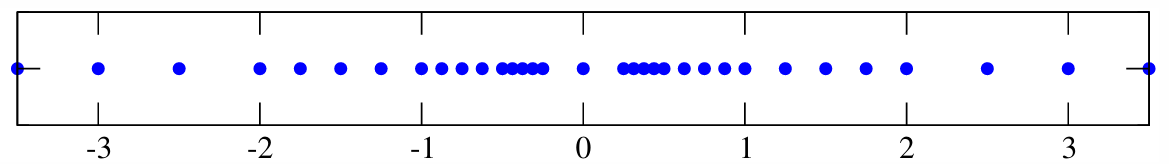
\includegraphics[width=0.75\textwidth]{rapp.png}
                \end{center}

            \end{enumerate}

            \subsubsection*{Nel calcolatore}
            
            Nel calcolatore la base è chiaramente 2, le cifre utilizzate sono $0$ e $1$

            Per codificare un numero macchina $x = (-1)^s (0.d_1d_2...d_t)B^e$ è sufficiente memorizzare:

            \begin{itemize}
                \item Il segno, costituito da un bit
                
                \item Le cifre della mantissa, costituite da $t$ bit
                
                \item L'esponente
            \end{itemize}
                
            Ogni numero macchina è rappresentato in 3 diverse forme:

            \begin{enumerate}
                \item Precisione singole (single precision), da $32$ bit
                
                \item Precisione doppia (double precision), da $64$ bit
                
                \item Precisione mezza (half precision), dal 2008 per l'utilizzo delle GPU, da $16$ bit
                
            \end{enumerate}
                    
        \subsubsection{Single Precision}
            I numeri macchina a precisione singola occupano 32 bit: 
            \begin{itemize}
                \item 1 bit per il segno 
                
                \item 8 bit per l'esponente
                
                \item 23 bit per la mantissa
                
            \end{itemize}
            
            Attualmente l'insieme dei numeri macchina in singola precisione è $\mathbb{F}(2, 24, -126, 127)$.

            \paragraph{}
            Il numero 24 di bit per la mantissa deriva dal bit nascosto: nella rappresentazione floating point normalizzata la prima cifra dopo la virgola è diversa da $0$, il che implica che in base due è $1$. Assumendo ciò non avrebbe senso rappresentare quella cifra sprecando un bit, che lo si usa invece per rappresentare una cifra in più per la mantissa.  

            \paragraph{}
            Nell'esponente, avendo 8 bit si possono rappresentare $2^8 = 256$ esponenti possibili, metà pari e metà dispari.
            Di quei 256, 2 sono riservati per uso speciale: 

            \begin{itemize}
                \item rappresentazione di infinito: mantissa = 0, esponente 0 o 1, seguito dal massimo esponente possibile, 1111111 
                \item NaN, Not a Number: mantissa $\neq$ 0, sponente 0 o 1 seguito dal massimo esponente possibile, 1111111
            \end{itemize}

            \paragraph{}
            I numeri rappresentabili in singola precisione sono:


            \[
                2(U-L+1)(B-1)B^{t-1}+1 = 2\cdot254\cdot1\cdot2^{23} + 1 \approx 4.2789 \cdot 10^9
            \]



            \subsubsection{Double Precision}

            I numeri macchina a precisione doppia occupano 64 bit: 

            \begin{itemize}
                \item 1 bit per il segno
                \item 11 bit per l'esponente
                \item 52 bit per la mantissa
            \end{itemize}
            
            L'insieme dei numeri macchina in precisione doppia è $\mathbb{F}(2, 53, -1022, 1023)$.

            \paragraph{}
            Il numero 53 di bit per la mantissa deriva dal bit nascosto, come per la precisione singola.

            Nell'esponente, avendo 11 bit si possono rappresentare $2^{11} = 2048$ esponenti possibili, metà pari e metà dispari.
            Di quei 2048, 2 sono riservati per uso speciale: 

            \begin{itemize}
                \item rappresentazione di infinito: mantissa = 0, esponente 0 o 1, seguito dal massimo esponente possibile, tutti bit a 1
                \item NaN, Not a Number: mantissa $\neq$ 0, sponente 0 o 1 seguito dal massimo esponente possibile, tutti i bit a 1
            \end{itemize}

            \paragraph{}
            I numeri rappresentabili in doppia precisione sono:



            \[
                2(U-L+1)(B-1)B^{t-1}+1 = 2\cdot 2046\cdot1\cdot2^{52}+1 \approx 1.8438\cdot 10^{19}
            \]



            \subsubsection{Half Precision}

            I numeri macchina ad half precision occupano 16 bit; l'utilizzo di così pochi bit permette di eseguire i calcoli molto più velocemente, fondamentale per le GPU:

            \begin{itemize}
                \item 1 bit per il segno 
                \item 5 bit per l'esponente
                \item 10 bit per la mantissa
            \end{itemize}
            
            L'insieme dei numeri macchina in precisione doppia è $\mathbb{F}(2, 11, -14, 15)$.

            \paragraph{}
            Il numero 10 di bit per la mantissa deriva dal bit nascosto, come per la precisione singola e doppia.

            Nell'esponente, avendo 5 bit si possono rappresentare $2^5 = 32$ esponenti possibili, metà pari e metà dispari.
            Di quei 32, 2 sono riservati per uso speciale:

            \begin{itemize}
                \item rappresentazione di infinito: mantissa = 0, esponente 0 o 1, seguito dal massimo esponente possibile, tutti bit a 1
                \item NaN, Not a Number: mantissa $\neq$ 0, sponente 0 o 1 seguito dal massimo esponente possibile, tutti i bit a 1
            \end{itemize}

            I numeri rappresentabili nella half precision sono:



            \[
                2(U-L+1)(B-1)B^{t-1}+1 = 2\cdot 30\cdot1\cdot2^{10}+1 \approx 6.1440\cdot 10^{4}
            \]


            
        \subsection{Approssimazione}

        In $\mathbb{F}(B,t,L,U)$ quando un numero $x= pB^e \in \mathbb{R}$ ha più di $t$ cifre nella mantissa
        (con esponente $L$ e $U$) può venire approssimato con un numero macchina, che chiameremo $fl(x)$, in due modi possibili:

        \begin{itemize}
            \item TRONCAMENTO: 
            
            Nella mantissa p si cancella la parte che eccede la t-esima cifra.


            \item ARROTONDAMENTO:
            
            Nella mantissa p si aggiunge $\frac{B}{2}B^{-(t+1)}$ e poi si tronca alla t-esima cifra

        \end{itemize}

        es. con t = 6, per troncamento: 



        \begin{align}
            x &= 0.745645897 \notag \\
            fl(x) &= tr(x) = tr(0.745645897) \notag \\
            &= 0.745645 \notag
        \end{align}



        Si noti che arrotondare equivale a sommare 1 alla t-esima cifra della mantissa, $d_{t}$, se la successiva cifra $(d_{t+1})$ è $\geq \frac{B}{2}$, altrimenti la cifra t-esima rimane invariata.

        \subsection{Underflow e Overflow}

        In $\mathbb{F}(B,t,L,U)$, nell’approssimare x con $fl(x)$ 

        \begin{itemize}
            \item se l’esponente $e > U$, si produce un Overflow. Il numero x viene
            rappresentato come Inf. (Più grave)
            \item se l’esponente $e < L$, si produce un Underflow. Il numero x viene
            rappresentato come 0.
        \end{itemize}

        OSS: una pratica per evitare l'overflow è quella di separare i calcoli

        \subsection{Errori Assoluti e relativi}

        Se $x$ è un numero reale e $x^*$ una sua approssimazione definiamo:

        ERRORE ASSOLUTO: la quantità $|x-x^*|$, in sè non da molta informazione

        ERRORE RELATIVO: la quantità $\frac{|x-x^*|}{|x|}$
        se $x\neq 0 $.

        \paragraph{}
        Nel caso si abbia a che fare con enti diversi da numeri reali (funzioni, vettori, matrici) le sono le stesse a patto di sostituire il valore assoluto con un’opportuna norma.

        L’errore relativo fornisce una indicazione più precisa della distanza fra $x$ e $x^*$.

        \paragraph{}

        Esempio. Siano $x = 0.456789\cdot10^{-30}$ e $x^* = 0.6 \cdot 10^{-30}$.

        \begin{itemize}
            \item Errore assoluto  $|x-x^*| = 0.143211\cdot10^{-30}$
            \item Errore relativo $\frac{|x-x^*|}{|x|} = 0.313517$
        \end{itemize}

        L’errore relativo è maggiore del 31\%!!

        \subsubsection{Errori assoluti di rappresentazione}

        \paragraph{}

        Sia $x \in \mathbb{R}$ e $fl(x) \in \mathbb{F}(B, t, U, L )$, allora:

        l'errore assoluto per troncamento è (trovo un upper bound):



        \begin{align}
            |x - fl(x)| &= |pB^e - \overline{p} B^e| \notag \\
            &= |p - \overline{p}| B^e \notag \\ 
            &\leq B^{-t} B^e \notag
        \end{align}

        più nello specifico: 

        \begin{align}
            p &= 0.d_1d_2...d_t... \notag \\
            \overline{p} &= 0.d_1d_2...d_t000 \notag \\ 
            \notag \\
            |p-\overline{p}| &= 0.0...0d_{t+1}d_{t+2}\notag \\
            &\leq 0.0...(B-1)(B-1)... \notag \\
            &= \sum_{k = t+1}^{\infty} (B-1)B^{-k} \notag \\
            &= B^{-t} \notag 
        \end{align}


        \textbf{Esempio:}

        \begin{itemize}
            \item $x =0.745645897$, $fl(x)=0.745645 $
            \[
                |x-fl(x)| = 0.000000897 = 0.897\cdot10^{-6} < 10^{-6}
            \]
        \end{itemize}


        L'errore assoluto per arrotondamento è: 



        \begin{align}
            \left| x - \text{fl}(x) \right| &= \left| pB^e - \bar{p}B^e \right| \notag \\
            &= \left| p - \bar{p} \right| B^e \notag \\
            &\leq \frac{B}{2} B^{-(t+1)} B^e \notag
        \end{align}

        più nello specifico distinguo due casi:

        \[
            \begin{cases}
                0.d_1d_2...d_td_{t+1}... \\
                0.d_1d_2...d_t
            \end{cases}
        \]    

        A: 
        \begin{align}
            d_{t+1} &\geq \frac{B}{2} \implies |p-\overline{p}| \leq \frac{B}{2}B^{-(t+1)} \notag
        \end{align}

        B:
        \begin{align}
            d_{t+1} &\leq \frac{B}{2} \quad \text{(applico troncamento)} \notag \\
            &\implies 0.d_1d_2\ldots d_t \left( \frac{B}{2} - 1 \right) (B-1)(B-1)\ldots \notag \\
            |p-\overline{p}| &= \left( \frac{B}{2} - 1 \right) B^{-(t+1)} + (B-1) \sum_{k = t+1}^{\infty} d_k B^{-k} \notag \\
            &= \left( \frac{B}{2} - 1 \right) B^{-(t+1)} + (B-1) \sum_{k = t+1}^{\infty} B^{-k} \notag \\
            &= \ldots \notag
        \end{align}
        
        
        
        



        \textbf{Esempio:}

        \begin{itemize}
            \item $x =0.745645897$, $fl(x)=0.745646 $
            \[
                |x-fl(x)| = 0.000000103 = 1.03\cdot10^{-7} < 5\cdot10^{-7}
            \]
        \end{itemize}



        \subsubsection{Errore relativi di rappresentazione}
        L'errore relativo per troncamento è: 



        \begin{align}
            \frac{\left| x - \text{fl}(x) \right|}{\left | x \right |} &= \frac{\left| pB^e - \bar{p}B^e \right|}{pB^e} \notag \\
            &= \frac{\left| p - \bar{p} \right|}{p} \notag \\
            &\leq \frac{B^{-t}}{B^{-1}} = B^{1-t} \notag
        \end{align}



        \paragraph{}
        L'errore relativo per arrotondamento è: 



        \begin{align}
            \frac{\left| x - \text{fl}(x) \right|}{\left | x \right |} &= \frac{\left| pB^e - \bar{p}B^e \right|}{pB^e} \notag \\
            &= \frac{\left| p - \bar{p} \right|}{p} \notag \\
            &\leq \frac{B}{2} \frac{B^{-(t+1)}}{B^{-1}} = \frac{1}{2} B^{1-t} \notag
        \end{align}



        Si nota subito che l'errore relativo per arrotondamento è la metà di quello per troncamento:
        difatti, attualmente, la maggior parte dei sistemi implementa la tecnica di arrotondamento perché produce mediamente errori più piccoli.

        \paragraph{def. PRECISIONE MACCHINA: }
        si chiama PRECISIONE MACCHINA e si denota con il simbolo $u$ (unit roundoff) la quantità:



        \[
            u = \frac{1}{2} B^{1-t} \text{   (massimo errore)}
        \]  



        Rappresenta  il massimo errore relativo che si
        commette nell’approssimare il numero reale $x$ con il suo corrispondente numero macchina $fl(x)$ per arrotondamento.

        \paragraph{}
        In  $\mathbb{F}(2, 24,-126,127)$, singola precisione, $u = 2^{-24}\approx5.96\cdot10^{-8}$

        \paragraph{}
        In  $\mathbb{F}(2, 53,-1022,1023)$, doppia precisione, $u = 2^{-53}\approx1.11\cdot10^{-16}$
        \paragraph{}
        In  $\mathbb{F}(2, 11,-14, 15)$, doppia precisione, $u = 2^{-11}\approx4.8828125\cdot10^{-4}$











        \break
        \subsection{Standard ANSI IEEE-754r}

        \paragraph{}
        Lo standard ANIS IEEE 754r è stato scritto nel 1985 e modificato nel 1989 e, più recentemente, nel 2008 e costituisce lo standard ufficiale per la rappresentazione binaria dei numeri
        all’interno del calcolatore e l’aritmetica di macchina (il nome dello standard
        in inglese “Binary floating point arithmetic for microprocessor systems”).

        Secondo lo standard un numero non nullo normalizzato si scrive come



        \[
            x =(-1)^s \cdot (1+f)\cdot2^{e^*-bias}
        \]
        


        La mantissa si rappresenta dunque come $1.d_1d_2...d_{\tau}$, dove $f = 0.d_1d_2...d_{\tau}$

        \paragraph{}
        $\tau$ identifica il numero di bit usati per codificare la parte frazionaria della
        mantissa. Il numero di cifre totali per la mantissa è $t = \tau + 1$.

        Il vero esponente del numero e si immagazzina in traslazione come $e^* = e + bias$.
        In questa maniera non serve un bit di segno per l’esponente (faccio una semplice traslazione a sinistra).

        Il bias in singola precisione vale $127$ mentre in doppia $1023$.
        
        Lo standard riserva due dei possibili valori per l’esponente per codificare due situazioni speciali:

        \begin{itemize}
            \item $e^* = 0$, viene riservato per la codifica dello zero ed eventuali numeri
            denormalizzati.
            \item $e^* = 255$ o $e^*=2047$, che corrisponde a un esponente vero pari a 128 (singola) o 1024 (doppia), viene riservato per la codifica di:
            
            \begin{enumerate}
                \item Inf (Overflow)
                \item NaN (Not a Number), ovvero operazioni del tipo $\frac{0}{0}$, $Inf-Inf$, $\frac{Inf}{Inf}$.
            \end{enumerate}

        \end{itemize}

        Il valore di $Inf$ viene codificato con mantissa nulla, mentre il valore $NaN$ corrisponde a mantissa $\neq 0$.

        \subsubsection*{Esempi: }
        
        Vediamo come si rappresenta il numero \( x = 126 \) secondo lo standard IEEE in singola precisione:
        \((126)_{10} = (1111110)_{2}\).
        Il numero \((1111110)_{2}\) si scrive, in virgola mobile normalizzata secondo lo standard IEEE, come:
            

        \[
            1.111110 \cdot 2^6
        \]


        Della mantissa si immagazzinano solo le cifre dopo la virgola.
        L'esponente normalizzato è:
            

        \[
            e^{*} = 6 + 127 = 133,
        \]


        che in binario corrisponde a:
            

        \[
            10000101.
        \]


        Il numero \( 126 \) viene codificato con la stringa:
            

        \[
            0 \quad 10000101 \quad 111111000000000000000000
        \]



        \subsection{Massimo e minimo rappresentabili}
        Sia $\mathbb{F}(B, t, L, U)$, quali sono il massimo e il minimo rappresentabili?

        \paragraph{}
        \textbf{MASSIMO: }
        Il numero più grande rappresentabile in aritmetica di macchina ha tutte le cifre della mantissa uguali a $B-1$ ed esponente $U$.

        \paragraph{}
        \textbf{Esempio: } in $\mathbb{F}(10, 6, L, U)$, sarebbe $0.999999\cdot10^U = (1-10^{-6}) \cdot 10^U$

        \paragraph{} Nello standard IEEE-754r in doppia precisione $\mathbb{F}(2, 53, -1022, 1023)$ il più grande valore rappresentabile è $(2-2^{52})\cdot2^1023 = 1.7977 \cdot 10^{308}$
        
        \paragraph{}
        \textbf{minimo: }
        Il più piccolo numero rappresentabile in aritmetica di macchina ha tutte le cifre della mantissa uguali a 0 tranne la prima (virgola mobile normalizzata) ed esponente L.
        
        \paragraph{}
        \textbf{Esempio: } in $\mathbb{F}(10,6,L,U)$, sarebbe $0.100000 \cdot 10^L = 10^{-1}\cdot 10^U$

        \paragraph{} Nello standard IEEE-754r in doppia precisione $\mathbb{F}(2, 53, -1022, 1023)$ il più piccolo valore rappresentabile è $ 1\cdot 2^{-1022} = 2.2251\cdot 10^{308}$



        \subsection{Distanza assoluta tra due numeri macchina}

        A differenza di quello che occorre in $\mathbb{R}$, in $\mathbb{F}$ la distanza tra $x$ e il suo elemento successivo $x_+$ non è infinitamente piccola, ma un valore ben determinato.
        \paragraph{def. } sia $x = (-1)^s(1+0.d_1d_2\cdots d_{\tau}) \cdot B^e$ e $x_+ = (-1)^s(1+0.d_1d_2\cdots (d_{\tau} + 1)) \cdot B^e$, la \textbf{distanza assoluta} tra $x$ e $x_+$ è:
        
        \begin{align}
            \Delta x = |x-x_+| = B^{-\tau} \cdot B^e = B^{e-\tau} \notag 
        \end{align}

        L'insieme dei numeri macchina è un insieme finito, questo implica che ci tale insieme dei numeri è "bucato": l'errore di rappresentazione è inevitabile. 

        La distanza assoluta tra un numero macchina e il suo successivo determina, dato $x \in \mathbb{R}$, i numeri sommabili "non visibili". 
        
        Se $x \in \mathbb{R}$ è compreso tra $fl(x)$ e $fl(x_+)$ tale numero $x$ non potrà essere rappresentato se non da $fl(x)$ o $fl(x_+)$, per troncamento o per arrotondamento. 

        Questa distanza è uguale per tutti i numeri macchina aventi lo stesso esponente.

        \paragraph{}
        L’incremento/decremento di una unità dell’esponente comporta un incremento/decremento di in fattore pari alla base della distanza assoluta tra due numeri macchina consecutivi.

        \paragraph{OSS: } Come visto in precedenza: i numeri macchina sono più addensati quanto più
        piccoli sono e la loro separazione aumenta man mano che aumenta il loro valore assoluto.
        


        \subsubsection{Distanza relativa}
        \paragraph{def. distanza relativa: } la distanza relativa tra x e il suo elemento successivo $x_+$ si ottiene dividendo  la distanza assoluta per il valore di x:

        \begin{align}
            \frac{|x-x_+|}{|x|} = \frac{B^{e-\tau}}{p\cdot B^e} = \frac{B^{-\tau}}{p} \notag
        \end{align}

        \paragraph{OSS: } Si può vedere che la distanza relativa tra due numeri macchina consecutivi ha
        un andamento periodico.

        \paragraph{} 
        Si può definire la massima distanza relativa tra due numeri macchina consecutivi come:

        \begin{align}
            \epsilon_M = B^{-\tau} \notag
        \end{align}

        che si ottiene quando la mantissa p è uguale a 1.
        \paragraph{OSS: } Nello standard IEEE-754r in doppia precisione $\epsilon_M = 2^{-52}$



        \subsubsection*{Precizione macchina (2)}
        A questo punto si può definire la precisione macchina come il massimo errore relativo di arrotondamento, che coincide anche con:

        \begin{align}
            u = \frac{\epsilon_M}{2} \notag
        \end{align}

        \paragraph{OSS:}
        In un computer che usa doppia precisione secondo lo standard IEEE-754r il valore della precisione di macchina è pari a $2^{-53} \approx 1.11 \cdot 10^{-16}$


        \subsection{Aritemtica macchina}

        Abbiamo visto che il numero $x$ non si rappresenta esattamente nel calcolatore ma si immagazzina come $fl(x)$ con un errore relativo massimo pari a
        $u = \frac{1}{2}B^{1-t}$.

        \paragraph{OSS: } 
        Come si propagano questi errori di rappresentazione quando si effettuano delle operazioni aritmetiche con i numeri macchina?

        Per distinguere le operazioni aritmetiche in $\mathbb{F}$ eseguite al calcolatore da quelle definite in $\mathbb{R}$, la seguente notazione:

        Dati \( x, y \) reali:

        \begin{itemize}
            \item Somma \( \oplus \):  $ x \oplus y = \text{fl}(\text{fl}(x) + \text{fl}(y))$ 


            \item Sottrazione \( \ominus \):  $ x \ominus y = \text{fl}(\text{fl}(x) - \text{fl}(y))$


            \item Prodotto \( \otimes \):  $ x \otimes y = \text{fl}(\text{fl}(x) \cdot \text{fl}(y)) $


            \item Divisione \( \oslash \):  $ x \oslash y = \text{fl}(\text{fl}(x) / \text{fl}(y)) $

        \end{itemize}

        \paragraph{OSS:} $fl(x)+fl(y)$ è la somma nel calcolatore, mentre $fl(fl(x)+fl(y))$ è il "trasferimento in memoria"

        \subsubsection*{Errori nelle operazioni macchina}
        
        Ricordiamo l'errore relativo di rappresentazione:

        \[
        \varepsilon_x = \frac{|x - \text{fl}(x)|}{|x|} \leq u.
        \]



        Definiamo ora l'errore relativo introdotto dalle operazioni macchina:


        \[
        \varepsilon^{\oplus}_{x,y} = \frac{|(x + y) - (x \oplus y)|}{|x + y|}
        \]


        Analogamente per le altre operazioni.

        Si può dimostrare che:


        \[
        \varepsilon^{\oplus}_{x,y} \leq \left| \frac{x}{x + y} \right| \varepsilon_x + \left| \frac{y}{x + y} \right| \varepsilon_y
        \]





        \[
        \varepsilon^{\otimes}_{x,y} \lesssim \varepsilon_x + \varepsilon_y
        \]





        \[
        \varepsilon^{\oslash}_{x,y} \leq \left| \varepsilon_x - \varepsilon_y \right|
        \]



        dove \(\varepsilon_x\) e \(\varepsilon_y\) sono tali che \(\varepsilon_x, \varepsilon_y \leq u\).

        \subsubsection{Errori nelle operazioni macchina: addizione}

        Dimostrazione di:


        \[
        \varepsilon^{\oplus}_{x,y} \leq \left| \frac{x}{x+y} \right| \varepsilon_x + \left| \frac{y}{x+y} \right| \varepsilon_y
        \]


        \pagebreak
        Assumiamo:


        \[
        x \neq 0, \quad y \neq 0, \quad x + y \neq 0, \quad \text{e} \quad \text{fl}(\text{fl}(x) + \text{fl}(y)) = \text{fl}(x) + \text{fl}(y),
        \]


        cioè la somma di \(\text{fl}(x)\) e \(\text{fl}(y)\) è un numero macchina. In caso contrario, la dimostrazione è più complicata ma l'enunciato rimane vero.



        \[
        \varepsilon^{\oplus}_{x,y} = \frac{|(x + y) - (x \oplus y)|}{|x + y|}
        = \frac{|(x + y) - (\text{fl}(x) + \text{fl}(y))|}{|x + y|}
        \]



        Applicando la disuguaglianza triangolare:


        \[
        \leq \frac{|(x - \text{fl}(x))|}{|x + y|} + \frac{|(y - \text{fl}(y))|}{|x + y|}
        \]



        Moltiplicando e dividendo per \(|x|\) e \(|y|\):


        \[
        = \frac{|(x - \text{fl}(x))| |x|}{|x + y| |x|} + \frac{|(y - \text{fl}(y))| |y|}{|x + y| |y|}
        \]



        Utilizzando la definizione di errore relativo:


        \[
        = \frac{|(x - \text{fl}(x))|}{|x|} \frac{|x|}{|x + y|} + \frac{|(y - \text{fl}(y))|}{|y|} \frac{|y|}{|x + y|}
        = \varepsilon_x \left| \frac{x}{x + y} \right| + \varepsilon_y \left| \frac{y}{x + y} \right|
        \]

        
        \subsubsection{Errori nelle operazioni macchina: prodotto}

        Stesse ipotesi: assumiamo \( x \neq 0, y \neq 0, x \cdot y \neq 0 \), e


        \[
        \text{fl}(\text{fl}(x) \cdot \text{fl}(y)) = \text{fl}(x) \cdot \text{fl}(y),
        \]


        ossia il prodotto di \(\text{fl}(x)\) e \(\text{fl}(y)\) è già arrotondato.

        Dimostrazione (analoga) di:


        \[
        \varepsilon^{\otimes }_{x,y} \lesssim \varepsilon_x + \varepsilon_y.
        \]



        L'errore relativo del prodotto macchina è definito da:


        \[
        \varepsilon^{\otimes }_{x,y} = \frac{|(x \cdot y) - (x \otimes y)|}{|x \cdot y|}.
        \]



        Passaggi:


        \[
        \varepsilon^{\otimes }_{x,y} = \frac{|(x \cdot y) - \text{fl}(\text{fl}(x) \cdot \text{fl}(y))|}{|x \cdot y|},
        \]




        \[
        = \frac{|(x \cdot y) - (\text{fl}(x) \cdot \text{fl}(y))|}{|x \cdot y|},
        \]




        \[
        = \frac{|x \cdot y - x \cdot \text{fl}(y) + x \cdot \text{fl}(y) - \text{fl}(x) \cdot \text{fl}(y)|}{|x \cdot y|}.
        \]


        \[
        = \frac{|x \cdot (y-\text{fl}(y)) + (x -\text{fl}(x)) \cdot \text{fl(y)}|}{|x \cdot y|}.
        \]
    



        Utilizzando la disuguaglianza triangolare:


        \[
        \leq \frac{|x \cdot (y - \text{fl}(y))|}{|x \cdot y|} + \frac{|(x - \text{fl}(x)) \cdot \text{fl}(y)|}{|x \cdot y|}.
        \]



        Assumendo che \( \text{fl}(y) / y \approx 1 \), diventa:


        \[
        = \frac{|y - \text{fl}(y)|}{|y|} + \frac{|x - \text{fl}(x)|}{|x|}.
        \]



        Quindi otteniamo:


        \[
        \varepsilon^{\otimes }_{x, y} \lesssim \varepsilon_x + \varepsilon_y.
        \]


        \subsubsection*{Osservazioni sugli errori macchina}

        Le operazioni macchina, come il prodotto e la divisione, introducono un errore relativo dell'ordine della precisione di macchina \( u \):


        \[
        \varepsilon_{x,y}^{\otimes} \approx \varepsilon_x + \varepsilon_y.
        \]

        \[
        \varepsilon_{x,y}^{\ominus} \leq |\varepsilon_x - \varepsilon_y|.
        \]



        Tuttavia, per la somma o la sottrazione, non si può garantire un errore relativo piccolo. In particolare:


        \[
        \varepsilon_{x,y}^{\oplus} \leq  \frac{|x|}{|x+y|} \varepsilon_x + \frac{|y|}{|x+y|} \varepsilon_y 
        \]


        il quale può diventare grande quando \( x \approx -y \). Questo fenomeno è noto come \textbf{Cancellazione numerica}. 

        Quindi, quando \( x \approx -y \), il risultato della somma (o sottrazione) è molto piccolo rispetto ai termini individuali, si amplifica l'effetto degli errori relativi di rappresentazione di \( x \) e \( y \).

        \textbf{Nota}: Questo è considerato una delle principali fonti di instabiltà

        \subsubsection{Cancellazione numerica}

        La cancellazione numerica si verifica come perdita di cifre significative nel risultato dovuto alla sottrazione di due numeri quasi uguali.

        \subsubsection*{Esempio}

        Consideriamo, in \( \mathbb{F}(10,5,*,*) \), i numeri:


        \[
        a = 0.73415507 \quad \text{e} \quad b = 0.73415448 \text{, essi sono qusi uguali}
        \]



        Nell'aritmetica di macchina:


        \[
        \text{fl}(a) = 0.73416, \quad \text{fl}(b) = 0.73415.
        \]



        Calcoliamo:


        \[
        a - b = 0.59 \cdot 10^{-6} \quad \text{(valore esatto)}.
        \]



        Nell'aritmetica di macchina:


        \[
        \text{fl}(\text{fl}(a) - \text{fl}(b)) = 0.00001 = 10^{-5}.
        \]



        L'errore relativo è dato da:


        \[
        \left| \frac{(a - b) - (a \ominus b)}{a - b} \right| = \frac{0.59 \cdot 10^{-6} - 10^{-5}}{0.59 \cdot 10^{-6}} = \frac{0.941 \cdot 10^{-5}}{0.59 \cdot 10^{-6}} = 15.949 \approx 1595 \%.
        \]



        La precisione di macchina in questa aritmetica è:


        \[
        u = \frac{1}{2} B^{1-t} = \frac{1}{2} 10^{-4} = 5 \cdot 10^{-5}.
        \]

        con una differenza in grandezza di un ordine di $10^8$.



        \textbf{Obiettivo}: Arrivare ad avere un errore pari alla precisione di macchina.
                

        \subsubsection*{Cancellazione numerica: esempio}

        Anche in casi non clamorosi come il precedente, l'errore può comunque essere molto maggiore della precisione di macchina.

        Sia l'aritmetica di macchina \( \mathbb{F}(10, 6, *, *) \). Consideriamo:


        \[
        a = 0.147554326, \quad b = 0.147251742.
        \]



        Naturalmente:


        \[
        \text{fl}(a) = 0.147554, \quad \text{fl}(b) = 0.147252.
        \]



        Calcoliamo la differenza esatta:


        \[
        a - b = 0.000302584 \quad \text{(valore esatto)}.
        \]



        Nell'aritmetica di macchina:


        \[
        a \ominus b = 0.000302.
        \]



        Errore relativo:


        \[
        \frac{|(a - b) - (a \ominus b)|}{|a - b|} = \frac{0.000302584 - 0.000302}{0.000302584} \approx 1.9 \cdot 10^{-3} \approx 0.19\%.
        \]



        Precisione di macchina:


        \[
        u = \frac{1}{2} B^{1-t} = \frac{1}{2} 10^{-5} = 5 \cdot 10^{-6}.
        \]



        \textbf{OSS}: il problema della cancellazione numerica si verifica quando i due numeri (sommati o sottratti) sono molto simili $\implies$ non è sempre un problema

        \paragraph{Violazione della proprietà associativa nelle operazioni macchina: }

        La proprietà associativa non è valida nelle operazioni in aritmetica floating-point \( F \). Questo implica che, in generale:


        \[
        (a \oplus b) \oplus c \neq a \oplus (b \oplus c).
        \]



        \subsubsection*{Esempio: }
        Consideriamo i numeri: $ (1 \oplus 10^{-15}) \oplus 1 \quad \text{e} \quad (1 \oplus 1) \oplus 10^{-15}. $



        Calcoliamo:


        \[
        (1 \oplus 10^{-15}) \oplus 1 = 1.11 \cdot 10^{-15}
        \]




        \[
        (1 \oplus 1) \oplus 10^{-15} = 10^{-15}
        \]



        L'ordine delle operazioni influenza in modo significativo il risultato.

        \subsubsection*{Esempio: Overflow o Underflow}
        Quando i numeri diventano molto grandi o molto piccoli, si possono verificare fenomeni di \textit{overflow} o \textit{underflow}. Ad esempio $a = 1.0 \cdot 10^{308}, \quad b = 1.1 \cdot 10^{308}, \quad c = -1.001 \cdot 10^{308}. $


        Calcoliamo:


        \[
        a \oplus (b \oplus c) = 1.0 \cdot 10^{308} \oplus (0.99 \cdot 10^{307}) = 1.099 \cdot 10^{308}
        \]




        \[
        (a \oplus b) \oplus c = \infty \oplus c = \infty
        \]



        \textbf{Nota}: L'ordine delle operazioni può portare a risultati non confrontabili.
                


        \subsubsection*{Cancellazione numerica e stabilità di un algoritmo}

        \textbf{def. }Un metodo numerico (formula, algoritmo) si dice \textbf{stabile} se \textit{non propaga gli errori (inevitabili) dovuti alla rappresentazione dei numeri nel calcolatore.} Altrimenti si dice \textbf{instabile}.

        \paragraph{}
        \textbf{OSS: }
        \begin{itemize}
            \item La cancellazione numerica genera delle formule instabili.
            \item Per evitare i problemi legati alla cancellazione numerica occorre trasformare le formule in altre numericamente più stabili.
            \item La stabilità è un concetto legato all’algoritmo usato per risolvere un determinato problema.
        \end{itemize}

        \textbf{OSS: } Una formula può essere instabile anche per altre cause, NON SOLO per cancellazione numerica!!!
        
        \paragraph{}
        La cancellazione numerica è un problema che si verifica durante l'operazione su numeri con differenze significative di ordine di grandezza. Questo può essere affrontato attraverso metodi alternativi per rendere l'algoritmo più stabile.

        \paragraph{}
        \textbf{Esempio: }

        Consideriamo la seguente operazione:


        \[
        \sqrt{x + \delta} - \sqrt{x}, \quad \text{per} \quad \delta \to 0
        \]



        Questa formula subisce cancellazione numerica. Si può risolvere razionalizzandola:


        \[
        \sqrt{x + \delta} - \sqrt{x} = \frac{\sqrt{x + \delta} + \sqrt{x}}{\sqrt{x + \delta} + \sqrt{x}} = \frac{\delta}{\sqrt{x + \delta} + \sqrt{x}}
        \]


        \paragraph{}
        \textbf{Esempio: in doppia precisione}

        Calcoliamo:


        \[
        \sqrt{1 + 10^{-14}} - \sqrt{1} = 4.88498130835069 \cdot 10^{-15}
        \]


        con un errore relativo di \(0.023 = 2.3\%\).

        Usando la formula stabile:


        \[
        \frac{10^{-14}}{\sqrt{1 + 10^{-14}} + \sqrt{1}} = 4.999999999999999 \cdot 10^{-15}
        \]


        con un errore relativo relativo di \(1.58 \cdot 10^{-16}\).

        \subsubsection*{Esempio di algoritmo instabile}

        \textbf{Formula risolutiva dell'equazione di secondo grado}

        Si vuole risolvere l'equazione:


        \[
            ax^2 + bx + c = 0 \quad \text{con} \quad a \neq 0
        \]



        Dividendo per \(a\), otteniamo:


        \[
            x^2 + \frac{b}{a}x + \frac{c}{a} = 0
        \]



        Ponendo:


        \[
        \frac{b}{a} = 2p \quad \text{e} \quad \frac{c}{a} = -q
        \]


        l'equazione si trasforma in:


        \[
        x^2 + 2px - q = 0
        \]



        La formula risolutiva per un'equazione quadratica calcola le due radici come:


        \[
        x_{1,2} = \frac{-2p \pm \sqrt{4p^2 + 4q}}{2}
        \]



        Semplificando:


        \[
        x_{1,2} = -p \pm \sqrt{p^2 + q}
        \]



        Se \(q\) è molto piccolo rispetto al termine quadratico \(p^2\), i risultati possono essere numericamente instabili. Ciò può portare a cancellazione numerica quando \(q\) viene sommato o sottratto a \(p^2\).

        \paragraph{}
        Consideriamo ora l'equazione quadratica:


        \[
        x^2 + 2px - q = 0
        \]


        con la condizione \(p^2 + q \geq 0\), che garantisce radici reali.

        La radice \(x_1\) viene calcolata con la seguente formula:


        \[
        x_1 = -p + \sqrt{p^2 + q}
        \]



        \paragraph{Problema di instabilità: }
        La formula diventa instabile se \(p \gg q > 0\), a causa della possibile cancellazione numerica tra \(p\) e \(\sqrt{p^2 + q}\).

        \subsubsection*{Soluzione alternativa}
        Per evitare l'instabilità numerica, possiamo razionalizzare la formula. Moltiplicando numeratore e denominatore per \(p + \sqrt{p^2 + q}\), otteniamo:


        \begin{align}
            x_1 &= \frac{(-p + \sqrt{p^2 + q})(p + \sqrt{p^2 + q})}{p + \sqrt{p^2 + q}} \notag \\
            x_1 &= \frac{q}{p + \sqrt{p^2 + q}} \notag
        \end{align}
        
        

        Questa forma è numericamente più stabile e riduce il rischio di cancellazione.


        \subsubsection*{Esempio: }
        Si vuole risolvere l'equazione:


        \[
        x^2 - 2px + 10^{-2} = 0
        \]


        per valori di \( p \) crescenti: \( p = 10^4, 10^5, 10^6, 10^7, 10^8 \).

        Utilizzando la formula quadratica in doppia precisione (calcolata in Matlab), otteniamo la seguente tabella:



        \[
        \begin{array}{cccc}
        p & x_1 & x_1 \text{ vera} & \text{ERR. REL} \\
        1.0e+04 & 5.0000016927e-07 & 4.9999999999e-07 & 3.4e-07 \\
        1.0e+05 & 5.0000380725e-08 & 5.0000000000e-08 & 7.6e-06 \\
        1.0e+06 & 5.0058588386e-09 & 5.0000000000e-09 & 1.2e-03 \\
        1.0e+07 & 0.0000000000e+00 & 5.0000000000e-10 & 1.0e+00 \\
        1.0e+08 & 0.0000000000e+00 & 5.0000000000e-11 & 1.0e+00 \\
        \end{array}
        \]



        \subsubsection*{Osservazioni}
        I risultati evidenziano che:
        \begin{itemize}
            \item Per valori di \( p \) crescenti, la cancellazione numerica compromette i calcoli.
            \item Errori relativi \textbf{gravi} emergono per \( p = 10^7 \) e \( p = 10^8 \), dove si ottiene \( x_1 = 0 \) anziché il valore corretto.
        \end{itemize}


        \subsubsection*{Esempio di algoritmo instabile}

        In questo esempio, si vuole approssimare il valore di \( \pi \) utilizzando una formula ricorsiva. Questo processo può diventare instabile a causa di errori di arrotondamento accumulati a ogni iterazione.

        La formula per la successione \( z_n \) è data da:


        \begin{align}
            z_2 &= 2 \notag \\
            z_{n+1} &= 2^{n - 0.5} \sqrt{1 - \sqrt{1 - 4^{1-n}z_n^2}}, \quad n = 2, 3, \dots \notag 
        \end{align}     



        Dove $r = 4^{1-n}z_n^2$



        Questa formula dovrebbe teoricamente convergere al valore di \( \pi \). Tuttavia, errori numerici possono influire negativamente sulla convergenza.

        \paragraph{}
        \textbf{Analisi dei risultati: }

        La tabella seguente mostra i valori calcolati per alcuni passi dell'iterazione:



        \[
        \begin{array}{cccccc}
        n+1 & r & 1 - \sqrt{1 - r} & z_{n+1} & \frac{|z_{n+1} - \pi|}{\pi} \\
        \hline
        10 & 1.505\cdot10^{-4} & 7.529\cdot10^{-5} & 3.14157294036 & 6.27\cdot10^{-6} \\
        11 & 3.764\cdot10^{-5} & 1.882\cdot10^{-5} & 3.14158772527 & 1.57\cdot10^{-6} \\
        12 & 9.412\cdot10^{-6} & 4.706\cdot10^{-6} & 3.14159142150 & 3.92\cdot10^{-7} \\
        13 & 2.353\cdot10^{-6} & 1.176\cdot10^{-6} & 3.14159234561 & 9.08\cdot10^{-8} \\
        14 & 5.882\cdot10^{-7} & 2.941\cdot10^{-7} & 3.14159257654 & 2.45\cdot10^{-8} \\
        \vdots & \vdots & \vdots & \vdots & \vdots \\
        28 & 2.220\cdot10^{-15} & 1.110\cdot10^{-15} & 3.16227766016 & 6.58\cdot10^{-3} \\
        29 & 5.551\cdot10^{-16} & 3.330\cdot10^{-16} & 3.46410161513 & 1.03\cdot10^{-1} \\
        30 & 1.665\cdot10^{-16} & 1.110\cdot10^{-16} & 4.00000000000 & 2.73\cdot10^{-1} \\
        31 & 5.551\cdot10^{-17} & 0.000\cdot10^{0} & 0.00000000000 & 1.00\cdot10^{0} \\
        32 & 0.000\cdot10^{0} & 0.000\cdot10^{0} & 0.00000000000 & 1.00\cdot10^{0} \\
        \end{array}
        \]



        \subsubsection*{Commenti sui risultati}

        - **Convergenza iniziale**: Nei primi passi, i valori \( z_{n+1} \) si avvicinano rapidamente a \( \pi \), con un errore relativo decrescente.
        - **Instabilità numerica**: Dopo un certo numero di iterazioni, gli errori di arrotondamento accumulati portano a risultati significativamente errati. Ad esempio, per \( n+1 = 30 \), il valore diverge completamente.
        - **Problema finale**: Nei passi finali, la successione collassa a zero, indicando un fallimento dell'algoritmo.

        \subsubsection*{Grafico del comportamento: }

        \begin{figure}[h!] 
            \centering 
            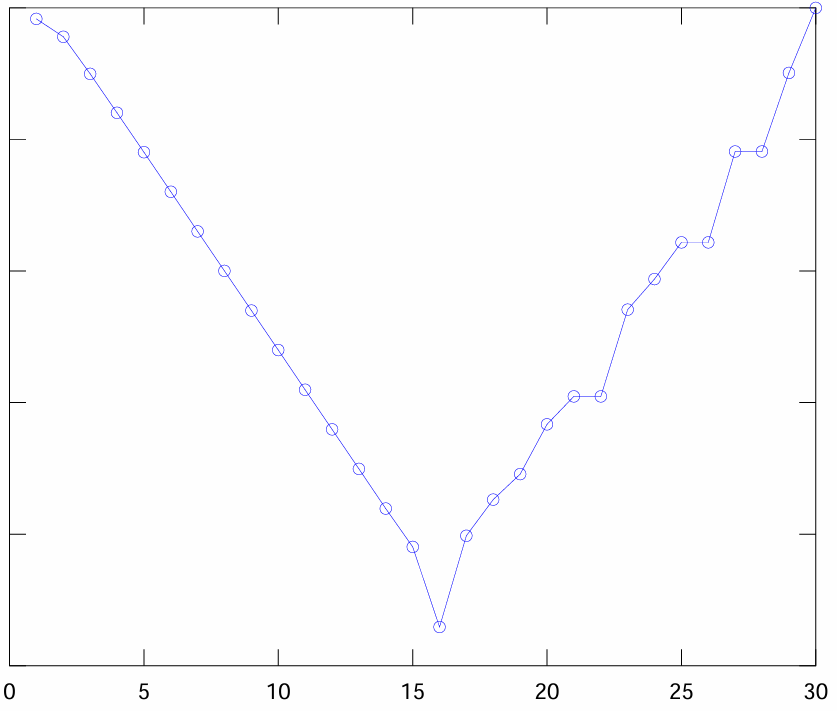
\includegraphics[width=0.5\textwidth]{graph1.png} 
        \end{figure}

        Il grafico seguente illustra come l'errore relativo \( \frac{|z_{n+1} - \pi|}{\pi} \) varia al crescere di \( n+1 \). Si osserva che l'errore aumenta drasticamente dopo un certo numero di iterazioni, a causa dell'accumulo degli errori numerici.

        \subsubsection*{Esempio di algoritmo instabile}
        

        Consideriamo la successione di integrali definiti \( I_n \), data da:


        \begin{align}
            I_n &= \frac{1}{e} \int_{0}^{1} x^n e^x \, dx, \quad n \geq 0 \notag \\
            \text{dove } I_0 &= \frac{1}{e} \int_{0}^{1} e^x \, dx = \frac{1}{e} \big[ e^x \big]_0^1 = 1 - \frac{1}{e} \approx 0.632121 \notag
        \end{align}
        

       Per \( n \geq 1 \), utilizziamo l'integrazione per parti:


        \[
        u = x^n, \quad dv = e^x \, dx \implies du = n x^{n-1} \, dx, \quad v = e^x 
        \]



        Da cui:


        \[
        I_n = \frac{1}{e} \left( \big[ x^n e^x \big]_0^1 - \int_{0}^{1} n x^{n-1} e^x \, dx \right) = 1-nI_{n-1}
        \]



        E quindi fissato $I_0$, per $n \geq 1$:


        \[
            I_n = 1 - n I_{n-1}
        \]

        Si ottiene quindi che:

        \[
            (I_n)_n = 
            \begin{cases}
                1-\frac{1}{e}, \text{ n = 0} \\
                1 - nI_{n-1}, \text{ altrimenti}
            \end{cases}     
        \]
        \paragraph{OSS: } NON c'è cancellazone numerica
        \paragraph{OSS: } si noti che $0 \leq I_n \leq 1 \implies nI_{n-1} \neq 1$

        
        \paragraph{}
        Implementando tale formula per il calcolo di $I_n$,per $n = 2,\ldots,25$, si ottengono i valori plottati in modulo nel seguente grafico:

        \begin{figure}
            \centering 
            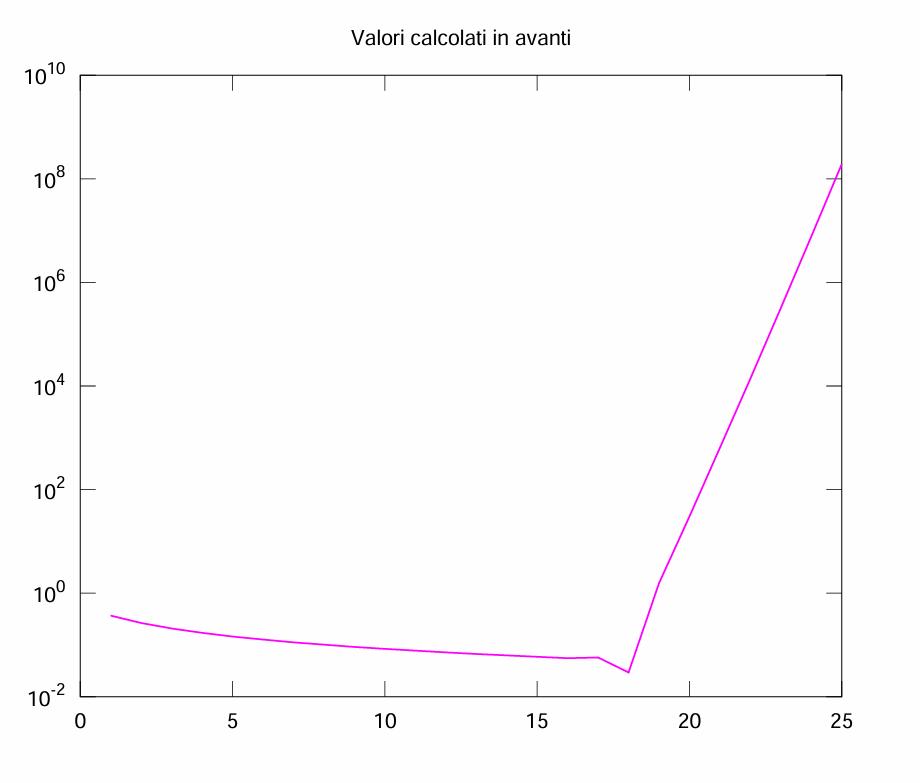
\includegraphics[width=0.7\textwidth]{graph2.png} 
        \end{figure}

        \paragraph{}
        La formula $I_n = 1-nI_{n-1}$ è instabile, quindi amplifica l’errore ad ogni passo, infatti nel calcolatore: 



        \[
            (I_n+\epsilon_n) = 1-(I_{n-1} + \epsilon_{n-1})
        \]

        
        
        Sottraendo dalla precedente equazione la relazione $I_n = 1-nI_{n-1}$ si può quantificare l’errore:


        \begin{align}
            \epsilon_n &= -n\epsilon_{n-1}, \text{ per induzione } \notag \\
            |\epsilon_n| &= n!|\epsilon_0| \notag
        \end{align}



        Il fattore $n!$ amplifica l'errore di rappresentazione iniziale (su $I_0$), $\epsilon_0$

        \paragraph{Esempio: } Nel calcolo di $I_{20}$ l’errore è $\epsilon_{20} = 20!\epsilon_0 \approx 2.7\cdot10^2$


        \subsubsection{Formula Alternativa stabile: }
        \textbf{Successione ricorrente all'indietro}

        \paragraph{} Il valore di $I_{m-k}$ si può calcolare a partire da una approssimazione di $I_m$ mediante
        questa formula all’indietro:
        


        \[
            I_{n-1}  =\frac{1}{n}(1-I+n), \text{ } n= m, m-1,\ldots, m-k+1
        \]

        che si ottiene dalla precedente ricavando $I_{n-1}$ in funzione di $I_n$.

        L'idea è di partire da un numero alto per andare fino ad un numero basso.

        Questa formula è stabile perchè l'errore ad ogni passo diminuisce anzichè aumentare.

        \paragraph{}
        L'errore al passo \( n-1 \) si trova come:


        \[
            \varepsilon_{n-1} = -\frac{1}{n} \varepsilon_n
        \]

        Partendo da \( m \)


        \[
        \begin{aligned}
            |\varepsilon_{m-1}| &= \frac{|\varepsilon_m|}{m} \\
            |\varepsilon_{m-2}| &= \frac{|\varepsilon_m|}{m(m-1)} \\
            &\;\vdots \\
            |\varepsilon_{m-k}| &= \frac{|\varepsilon_m|}{m(m-1)\cdots(m-k+1)}
        \end{aligned}
        \]

        \paragraph{}
        \textbf{Oss: } La produttoria al denominatore abbatte rapidamente l'errore iniziale!

        \paragraph{}
        \textbf{Esempio}
        Per calcolare \( l_{25} \) partendo da \( l_{40} = 0.5 \), l'errore iniziale \( |l_{40}| < 0.5 \) verrebbe abbattuto di un fattore:


        \[
        40 \cdot 39 \cdot \ldots \cdot 27 \cdot 26 = 5.2602 \cdot 10^{22}
        \]

        \subsection{Condizionamento}
        \textbf{def. }Un problema si dice \textbf{mal condizionato} se a piccole variazioni nei dati corrispondono grandi variazioni nei risultati.

        \begin{itemize}
            \item In caso contrario, il problema si dice \textbf{ben condizionato}.
            \item Il malcondizionamento è indipendente dall’algoritmo scelto per risolvere il problema: se il problema è mal condizionato, nessun algoritmo, per quanto stabile, potrà dare una soluzione corretta al problema stesso.
        \end{itemize}

        \paragraph{}
        \textbf{Esempio: }
        Consideriamo il problema di risolvere il sistema lineare:

        \[
            \begin{cases}
            x + y = 2 \\
            1001x + 1000y = 2001
            \end{cases}
        \]

        che ha come soluzione \( x = 1 \), \( y = 1 \).

        Se perturbiamo il coefficiente della \( x \) nella prima equazione di 0.01, otteniamo:

        \[
            \begin{cases}
            1.01x + y = 2 \\
            1001x + 1000y = 2001
            \end{cases}
        \]

        Il nuovo sistema ha come soluzione \( x = -0.11111111 \), \( y = 2.11222222 \) con un errore relativo su \( x \) e su \( y \) pari a:

        \[
            \text{err}_x = \frac{|1 + 0.11111111|}{1} = 1.11111111,
        \]

        \[
            \text{err}_y = \frac{|1 - 2.11222222|}{1} = 1.11222222
        \]

        entrambi maggiori del 100\%.


        \paragraph{}
        \textbf{def. numero di condizionamento } la quantità che misura il grado di sensibilità di un problema rispetto a piccole variazioni nei dati si dice \textbf{Numero di condizionamento}.

        \paragraph{}
        Consideriamo il problema di valutare una funzione di una variabile \( f \) in un punto: \( y = f(x) \).

        Se il dato di ingresso \( x \) è perturbato di una quantità \( \Delta x \), assumendo \( f \) derivabile, per il teorema di Lagrange:

        \[
            f(x + \Delta x) - f(x) = \Delta x f'(\xi)
        \]

        Detto \( \Delta y = f(x + \Delta x) - f(x) \) l'errore assoluto sul valore della funzione, quello relativo è:

        \[
            \left| \frac{\Delta y}{y} \right| = \left| \frac{\Delta x f'(\xi)}{y} \right| = \left| \frac{\Delta x}{x} \cdot \frac{x f'(\xi)}{y} \right|.
        \]

        Al limite, per \( \Delta x \to 0 \), \( \xi \to x \):

        \[
            \left| \frac{\Delta y}{y} \right| = K(f, x) \frac{|\Delta x|}{|x|}
        \]

        dove  $K(f, x) = \frac{|x f'(x)|}{|y|}$ è detto \textbf{Numero di condizionamento}.

        \paragraph{}
        \textbf{Esempio:}

        Data la funzione \( f(x) = \sqrt{1 - x^2} \), calcoliamo analiticamente il numero di condizionamento:


        \[
            K(f, x) = \frac{|x f'(x)|}{|y|} = \frac{|x \frac{-2x}{2\sqrt{1 - x^2}}|}{\sqrt{1 - x^2}} = \frac{x^2}{1 - x^2}
        \]



        Il problema sarà peggio condizionato quanto più \( x \) si approssima a 1:

        \[
        \begin{array}{c|c|c|c|c}
            x & 1 - 10^{-6} & 1 - 10^{-12} & 1 - 10^{-15} \\ \hline
            K(f, x) & 4.99999 \cdot 10^5 & 5.00011 \cdot 10^{11} & 5.0039996 \cdot 10^{14} \\
        \end{array}
        \]

        

    \section{Funzioni:}
        
        \paragraph{}
        Sia dato il problema: \( f(x) = 0 \), con \( f: I = [a, b] \to \mathbb{R} \), continua, allora il nostro obiettico sarà quello di trovare \( \alpha \in I$ $|$ $f(\alpha) = 0\); quindi si cercano gli zeri della funzione $f$ (radici di $f$) 
        
    
        \paragraph{}
        \textbf{Esempio:}
        \begin{align*}
            f(x) &= (x - 1)^2 = 0, \quad \text{$\alpha = +1$} \\
            f(x) &= \cos\left(\log\left(\frac{1}{x}\right)\right) = 0, \quad \text{$\alpha =  $}
        \end{align*}
           
        

        \paragraph{}
        \textbf{def. zero semplice}: sia $f(x)$ una funzione, allora $\alpha$ si dice \textbf{zero semplice} se $f(\alpha) = 0$ e $f'(\alpha) \neq 0 $, altrimenti ($f'(\alpha) = 0$) $\alpha$ si dice \textbf{multiplo}

        \paragraph{}
        \textbf{def. molteplicità di uno zero}: sia $f(x)$ una funzione, allora la molteplicità di uno zero è l'indice della prima derivata che non si annulla in $\alpha$.

        \paragraph{}
        \textbf{Esempio}: sia $f(x) = \cos{x}-1+\frac{x^2}{2}+\frac{x^5}{5}$

        Si nota che uno zero di $f$ è in $x = 0$; la derivata di $f$ in 0 però si annulla, pertanto $\alpha = x = 0$ è multiplo:

        \[ f'(x) = -\sin x + x + x^4 \quad ; \quad f'(0) = 0\]
        \[ f''(x) = -\cos x + 4x^3 \quad ; \quad f''(0) = 0\]
        \[ f^{(3)}(x) = \sin x + 12x^2 \quad ; \quad f^{(3)}(0) = 0 \]
        \[ f^{(4)}(x) = \cos x + 24x \quad ; \quad f^{(4)}(0) = 1 \neq 0 \]
        

        Quindi la molteplicità di uno zero è \( \tau = 4 \).

        \paragraph{}
        \textbf{th. esistenza dello zero:} sia \( f(x) \) continua in \([a,b]\) e tale che \( f(a)f(b) < 0 \), allora esiste \( \alpha \in [a,b] \) tale che \( f(\alpha) = 0 \).

        \paragraph{}
        \textbf{Condizione sufficiente per l'unicità dello zero:} se \( f(x) \) è monotona in senso stretto in \([a,b]\) ed $\exists$ \( \alpha \in [a,b] \) tale che \( f(\alpha) = 0 \), allora \( \alpha \) è unico.

        \paragraph{Esempio:}
        Consideriamo l'equazione: $f(x) = 2x^2 + \log(x) - \frac{1}{x} = 0$

        Esistenza: $f(0.1) = -12.28, \quad f(1) = 1 > 0 \implies$ esiste \( \alpha \in [0.1, 1] \) tale che \( f(x) = 0 \).

        Unicità: $f'(x) = 4x + \frac{1}{x} + \frac{1}{x^2} > 0 \quad \forall x \in [0.1, 1] \implies$ \( f \) è monotona crescente in \([0.1, 1]\), e quindi lo zero di \( f \) in \([0.1, 1]\) è unico.



        \subsection{Metodi Iterativi}
        Le procedure di calcolo di zeri di funzioni sono iterative.

        \paragraph{def. metodo iterativo:} un metodo iterativo è una procedura che a partire da un valore iniziale $x_0$ genera una successione \( \{x_k\}_{k \geq 0} \) a partire da uno o più termini precedenti.

        \paragraph{def convergenza di un metodo iterativo:} un metodo iterativo (o la successione  \( \{x_k\} \) da esso generata ) è convergente ad \( \alpha \) se:

        \[
            \lim_{k \to \infty} x_k = \alpha
        \]

        o equivalentemente se:

        \[
            \lim_{k \to \infty} | \alpha - x_k | = 0 \text{, con $|\alpha-x_k| = e_k$}
        \]

        (dove \( e_k \) è l'errore al passo \( k \)).

        \paragraph{def. convergenza locale:} un metodo iterativo converge localmente ad \( \alpha \) se esiste \( \delta > 0 \) tale che $ \forall  $ \( x_0 \in B(\alpha, \delta) = [\alpha - \delta, \alpha + \delta] \), si ha:

        \[
            \lim_{k \to \infty} x_k = \alpha.
        \]

        \paragraph{def. ordine di convergenza (di un metodo iterativo:)}sia $x_k$ un metodo iterativo convergente tale che \( x_k \to \alpha \) (la successione ha come limite \( \alpha \)), allora se esistono due costanti positive \( c \) e $p$ tali che:

        \[
            \lim_{k \to \infty} \frac{|e_{k+1}|}{|e_k|^p} = c, \quad c > 0, \quad p \geq 1, \quad p \in \mathbb{R}.
        \] 
        con $e_k = \alpha - x_k$, allora si dice che $x_k$ ha ordine di convergenza \( p \). 
        
        Se:        
        \begin{itemize}
            \item \( p = 1 \), allora il metodo iterativo $x_k$ ha convergenza lineare
            \[
                \lim_{k \to \infty} \frac{|e_{k+1}|}{|e_k|} = c \approx |e_{k+1}| \approx c \cdot |e_k|
            \]
            \item \( p = 2 \), allora il metodo iterativo $x_k$ ha convergenza quadratica:
            \[
                \lim_{k \to \infty} \frac{|e_{k+1}|}{|e_k|^2} = c \approx |e_{k+1}| \approx c \cdot |e_k|^2
            \]
            \item se \( p > 1 \), allora il metodo iterativo  $x_k$ ha convergenza superlineare.
        \end{itemize}

        \paragraph{def. costante asintotica di riduzione dell'errore:} per i metodi lineari, la costante \( c \) si chiama costante asintotica di riduzione dell'errore (fattore del quale si riduce l'errore asintoticamente).
        
        
        \paragraph{Oss. } Per \( p = 1 \), deve essere che \( c < 1 \), cosa non necessaria per $p = 2$
        


        \subsection{Metodo di Bisezione (Dicotomico)}
        Sia $f(x) = 0$, continua in \([a, b]\) e tale che esiste uno zero unico \( \alpha \in I = [a, b] \) tale che \( f(\alpha) = 0 \), si trovi $\alpha$

        \paragraph{Vantaggi:}
        \begin{itemize}
            \item Garantisce la convergenza se le ipotesi sono soddisfatte.
            \item È semplice da implementare.
        \end{itemize}

        \paragraph{Svantaggi:}
        \begin{itemize}
            \item La convergenza è lenta rispetto ad altri metodi come il metodo di Newton.
            \item Richiede che \( f(a)f(b) < 0 \), quindi non può essere applicato a funzioni che non soddisfano questa condizione.
        \end{itemize}

        \paragraph{Funzionamento: } genera una successione di intervalli $I_k$, chiusi, limitati e inscatolati di ragione la metà del precedente. Si ha inoltre che per ogni $I_k$ vale che $f(a_k)f(b_k) < 0$.

        \paragraph{Pseudocodice:}
        Dato $[a,b], f, f(a)f(b) < 0$, con $a_0 = a$, $b_0 = b$
        
        
        \begin{algorithm}
            \begin{algorithmic}[1]
            \State $x_k = \frac{a_k + b_k}{2}$
            \For{$k = 0, 1, \ldots$}
                \If{$f(x_k) = 0$}
                    \State \textbf{Fine}
                \ElsIf{$f(x_k) \cdot f(a_k) < 0$}
                    \State $b_k = x_k$
                \Else
                    \State $a_k = x_k$
                \EndIf
            \EndFor
        \end{algorithmic}
        \end{algorithm}

        \paragraph{}
        \textbf{Spiegazione: }
        Si calcola il punto medio per \( x_k = \frac{a_k + b_k}{2} \).
        Si valuta a questo punto \( f(x_k) \):
        \begin{itemize}
            \item Se \( f(x_k) = 0 \), allora \( x_k \) è lo zero cercato.
            \item Se \( f(a_k)f(x_k) < 0 \), allora lo zero si trova nell'intervallo \([a_k, x_k]\) e si pone $a_{k+1} = a_k$ e $b_{k+1} = x_k$
            \item Se \( f(x_k)f(b_k) < 0 \), allora lo zero si trova nell'intervallo \([x_k, b_k]\) si pone $a_{k+1} = a_k$ e $b_{k+1} = x_k$
        \end{itemize}
        Si ripete poi processo restringendo l'intervallo fino a ottenere una tolleranza desiderata \( \epsilon \), cioè \( |b_k - a_k| < \epsilon \).
        
        ($e_k = \alpha - x_k$ è l'errore al passo $k$, mentre $f(x_k)$ si dice residuo al passo k)

        \paragraph{Convergenza globale:}
        Il metodo di bisezione ha una convergenza globale, ad ogni iterazione, la lunghezza dell'intervallo si dimezza, quindi l'errore \( e_k \) al passo \( k \) è dato da:
        
        \[
            0 \le |e_k| \le \frac{b_k - a_k}{2} = \frac{b-a}{2^{k+1}}
        \]
        \paragraph{dim: } basta dimostrare che 

        \[
            \lim_{k \to +\infty} \frac{b-a}{2^{k+1}} = 0
        \]

        Per il teorema dei due carabinieri si ha che 

        \[
            \lim_{k \to +\infty} 0 = 0
        \]

        \[
            \lim_{k \to +\infty} \frac{b-a}{2^{k+1}} = 0
        \]

        Quindi 

        \[
            0 \leq |e_k| \leq \frac{b-a}{2^{k+1}}
        \]

        e quindi 

        \[
            \lim_{k \to +\infty} |e_k| = 0.
        \]

        \paragraph{Oss: } si noti l'ordine di convergenza e la costante asintotica: il metodo di bisezione ha come costanti $p = 1$ e $c = \frac{1}{2}$, ma se si calcola 

        \[
            \lim_{k \to +\infty} \frac{|e_{k+1}|}{|e_k|}
        \]
        NON esiste per il comportamento

        \subsubsection{Criterio di arresto}
        \paragraph{}
        \textbf{Test di arresto sul residuo}: Per arrestare le iterazioni, nel metodo della bisezione, posso considerare la semilunghezza dell'intervallo al passo k. 

        \paragraph{}
        Un criterio di arresto importante è quello basato sul \textbf{test di arresto sul residuo}: sia $e_k = \alpha - x_k$ l'errore al passo k, $f(\alpha) - f(x_k)$ è il residuo
        \paragraph{}
        \textbf{OSS: } problemi di arresto sul residuo:

        Il criterio di arresto basato sul residuo consiste nel fermare l'algoritmo iterativo quando il valore assoluto di \( f(x_k) \) è sufficientemente piccolo, ovvero \( |f(x_k)| < \text{tol} \), dove \(\text{tol}\) è una tolleranza prefissata. Tuttavia, questo criterio può essere problematico in alcune situazioni:

        \paragraph{}
        \textbf{Esempio funzione molto piatta:} consideriamo \( f(x) = 10^{-50}x \). Questa funzione è estremamente piatta, quindi anche per valori di \( x_k \) lontani dallo zero, il residuo \( f(x_k) \) può risultare molto piccolo. Ad esempio, se \( x_k = 10^{20} \), allora:
        \[
            f(x_k) = 10^{-50} \cdot 10^{20} = 10^{-30}.
        \]
        In questo caso, il residuo \( f(x_k) \) è molto piccolo, ma il valore di \( x_k \) è ancora lontano dalla radice \( \alpha = 0 \). Questo può portare a un arresto prematuro dell'algoritmo, senza aver raggiunto una soluzione accurata.

        \textbf{Esempio funzione molto ripida:} consideriamo \( f(x) = 10^{50}x \). Questa funzione è estremamente ripida, quindi anche per valori di \( x_k \) molto vicini alla radice, il residuo \( f(x_k) \) può risultare molto grande. Ad esempio, se \( x_k = 10^{-20} \), allora:
        \[
            f(x_k) = 10^{50} \cdot 10^{-20} = 10^{30}.
        \]
        In questo caso, il residuo \( f(x_k) \) è molto grande, ma il valore di \( x_k \) è già molto vicino alla radice \( \alpha = 0 \). Questo può portare a un prolungamento inutile dell'algoritmo, nonostante la soluzione sia già sufficientemente accurata.

        \paragraph{}
        \textbf{Soluzione: RESIDUO PESATO }
        si utilizza la quantità chiamata residuo pesato:

        \[
            \frac{f(x_k)}{f'(x_k)} \approx e_k + O(e_k^2) 
        \]

        Il residuzo pesato è una buona approssimazione di ordine 1 dell'errore
        
        \paragraph{Dim. } $e_k = \alpha - x_k$; \quad $\alpha = x_k + e_k$ 
        
        Scrivo lo sviluppo di Tyalor (utilizzando il resto di Lagrange): 

        \[
            0 = f(\alpha) = f(x_k + e_k) = f(x_k) + f'(x_k)e_k + O(e_k^2) 
        \]

        Assumendo che $f'(\alpha) \ne 0$ e che quindi $\alpha$ sia uno zero semplice
        
        \[
            \frac{-f(x_k)}{f'(x_k)} \approx e_k + O(e_k^2) \text{ dove $O(e_k^2)$ è trascurabile}
        \]

        \paragraph{Oss. } Si puà approssimare la derivata con il rapporto incrementale, perchè non si richiede che la fz. sia continua, quindi non è detto che la derivata esista. 


        \subsubsection{Numero Minimo di iterazioni}
        Il numero minimo di iterazioni per avere un errore inferiore a tol è:

        \[
            |e_k| < 10^{-t} = tol
        \]

        \[
            |e_k| \le \frac{b-a}{2^{k+1}} < tol   
        \]

        \[
            \log(b-a) - (k+1)\log_2 < \log(tol)
        \]

        \[
            \log(b-a) - \log_(tol) < (k+1)\log_2
        \]

        \[
            \frac{\log(b-a)-\log_(tol)}{\log_2} < (k+1)
        \]

        \[
            k > \frac{\log(b-a)-\log(tol)}{\log_2} -1
        \]
    

        \paragraph{}
        \textbf{Esempio:} $f(x) = e^{-2x}-x^2 = 0$, $I = [0,1]$
        
        \[
            \frac{1}{2^{k+1}} < 10^{-7}
        \]

        \[
            \frac{1}{10^{-7}} < 2^{k+1}
        \]

        \[
            k+1 > \log_2(10^7)
        \]

        \[
            k > 23.25 -1 \approx 23
        \]

        \paragraph{Esercizi: }

        \begin{align*}
            & \sin(x) - x = 0 \quad \\
            & 5x - e^{-x} = 0 \quad \\
            & x^2 - 5x + 6 = 0 \quad \\
            & e^{-\frac{x}{4}} - x = 0 \quad
        \end{align*}

        \subsection{Metodo Newton-Raphson}
        Applicabilità:
        \begin{itemize}
            \item \( f \in C^1([a,b]) \)
            \item \( \alpha \in [a,b] \mid f(\alpha) = 0 \)
        \end{itemize}

        \paragraph{}
        Funzionamento:

        Dato $x_0$ punto iniziale, il metodo di Newton approssima $f$ comn la retta tangente al $f$ in $(x_0, f(x_0))$, interseca la tangente con l'asse x. Il punto di intersezione è la nuova approssimazione dello zero. Poi si ripete la procedura.

        \paragraph{}
        Scehma iterativo: 
        Ci sono due modi per ricavarlo:
    
        \begin{enumerate}
            \item Traduzione matematica:
            suppongo di essere in \( x_k \):
            \[
            x_k = 
            \begin{cases}
                y = f(x_k)+f'(x_k)(x-x_k) \text{ (eq retta tangente)}\\
                y = 0
            \end{cases}
            \]

            \[
            \begin{aligned}
                0 = f(x_k) &+ f'(x_k)(x-x_k) \rightarrow \frac{-f(x_k)}{f'(x_k)} = x-x_k \rightarrow x = x_k - \frac{f(x_k)}{f'(x_k)} \\
                &x_{k+1} = x_k -\frac{f(x_k)}{f'(x_k)}, \quad k \geq 0
            \end{aligned}
            \]

            \item considero: $x_{k+1} = x_k + S$, dove $x_{k+1}$ è lo zero e $S$ è la differenza tra lo zero e il termine precedente

            utilizzo l'approssiazione di Tylor di $f$ attorno a $x_k$
            \[
                0 = f(x_{k+1}) = f(x_k+S) = f(x_k) + f'(x_k) S \quad \rightarrow -\frac{f(x_k)}{f'(x_k)} = S
            \]

            \[
                \rightarrow x_{k+1} = x_k + S = x_k-\frac{f(x_k)}{f'(x_k)}, \quad k \geq 0
            \]
        \end{enumerate}

        \paragraph{}
        \textbf{Th. di convergenza locale del Metodo di Newton-Raphson}: Sia \( f \in C^2([a,b]) \), con \( \alpha \in [a,b] \mid f(\alpha) = 0 \).
        Se \( f'(x) \neq 0 \, \forall x \in [a,b] \) (garantisce che lo zero sia semplice perchè $f'(\alpha) \neq 0$), allora esiste \( \delta > 0 \) tale che \( \forall x_0 \in B(\alpha, \delta) \):

        \begin{enumerate}
            \item il metodo è ben definito, \( \{x_k\}_{k \geq 0} \subset B(\alpha, \delta) \) $\rightarrow$ (la successione delle iterate è inclusa nella palla aperta di centro $\alpha$ e raggio $\delta$) 
            \item \( \frac{|e_{k+1}|}{|e_k|^2} < M \); (e quindi il limite \( k \to \infty \, x_k = \alpha \)) $\rightarrow$ (il rapporot tra errori è maggiorato da una costante) 
        \end{enumerate}

        Inoltre si ha convergenza quadrata:
        \[
            \lim_{k \to \infty} \frac{|e_{k+1}|}{|e_k|^2} = \frac{1}{2} \left| \frac{f''(\alpha)}{f'(\alpha)} \right|
        \]

        \paragraph{}
        \textbf{Dimostrazione: }
        \[
        e_k = \alpha - x_k; \quad \alpha = x_k + e_k;
        \]

        Utilizzando il resto di Lagrange: 
        \[
        0 = f(\alpha) = f(x_k + e_k) = f(x_k) + f'(x_k) e_k + \frac{1}{2} f''(\xi_k)e_k^2, \quad \xi_k \in \text{int}(x_k,\alpha)
        \]

        
        \[
            \text{Sapendo per ipotesi che $f'(x_k) \neq 0 \rightarrow$}-\frac{f(x_k)}{f'(x_k)} = e_k + \frac{1}{2} \frac{f''(\xi_k)}{f'(x_k)} e_k^2
        \]

        \[
            -\frac{f(x_k)}{f'(x_k)} = x_{k+1} - x_k =  e_k + \frac{1}{2} \frac{f''(\xi_k)}{f'(x_k)} e_k^2
        \]

        Sapendo che:
        \[
            x_{k+1} - \alpha + \alpha - x_k = e_k + \frac{1}{2} \frac{f''(\xi_k)}{f'(x_k)} e_k^2
        \]

        e:
        \[
            x_{k+1} - \alpha + \alpha - x_k = - e_{k+1} + e_k
        \]

        Divido per $e_k^2:$
        \[
        \frac{-e_{k+1}}{e_k^2} = \frac{1}{2} \frac{f''(\xi_k)}{f'(x_k)}
        \]
        Trovo che:
        \[
            \frac{|e_{k+1}|}{|e_k|^2} \leq \frac{1}{2} \frac{\max_{x \in [a,b]} |f''(x)|}{\min_{x \in [a,b]}|f'(x)|} = M
        \]

        Questo risultato ci permette di dimostrare la convergenza di \( x_k \) ad \( \alpha \) (ovvero che \(\lim_{k \to \infty} x_k = \alpha \iff \lim_{k \to \infty} |e_k| = 0\)).

        \[
            |e_{k+1}| \leq M |e_k|^2 \quad \rightarrow |e_k| \leq M |e_{k-1}|^2
        \]
        
        Moltiplico e divido per M:

        \[
            M|e_k| \leq (M |e_{k-1}|)^2 \leq (M|e_{k-2}|)^{2^2} \leq \ldots \leq (M|e_0|)^{2^k}
        \]

        Quindi:
        \[
            M(e_k) \leq (M|e_0|)^{2^k} \quad \rightarrow \quad 0 \leq |e_k| \leq \frac{1}{M} (M |e_0|)^{2^k}
        \]

        \[
            \Rightarrow x_0 \in \left( \alpha - \frac{1}{M}, \alpha + \frac{1}{M} \right) = B(\alpha, \delta) \quad \text{con} \quad \delta = \frac{1}{M}
        \]

        Partendo da $x_0 \in B(\alpha, \frac{1}{M})$, tutte le iterate restano dentro la palla $B \Rightarrow \{x_k\} \subset B(\alpha, \frac{1}{M})$
        \[
            x_k \in B(\alpha, \frac{1}{M}) \Rightarrow \underbrace{|\alpha - x_k|}_{e_k} < \frac{1}{M}
        \]

        Da $-\frac{e_{k+1}}{|e_k|^2} = \frac{1}{2} \frac{f''(\xi _k)}{f'(x_k)}$ passo al limite e ai valori assoluti:

        \begin{align*}
            \lim_{k \to \infty} \frac{|e_{k+1}|}{|e_k|^2} &= \frac{1}{2} \lim_{k \to \infty} \frac{|f''(xi_k)|}{f'(x_k)} = \frac{1}{2} \frac{f''(\lim_{k \to \infty} \xi_k)}{f'(\lim_{k \to \infty} x_k)} \text{ $\rightarrow$ (per continuità)} \\
            &= \frac{1}{2} \frac{|f''(\alpha)|}{|f'(\alpha)|}
        \end{align*}
            

        So che $x_k \to \alpha$, $\xi_k \in \text{int}(x_k, \alpha)$, quindi per $k \to \infty$, $\xi_k \to \alpha$.
                        
        \paragraph{}
        \text{Ordine di convergenza del metodo di Newton}
        
        \begin{itemize}
            \item se $f''(\alpha) \neq 0$, $c =\frac{1}{2} \left | \frac{f''(\alpha)}{f'(\alpha)} \right | \neq 0 \implies p = 2$
            \item se $f''(\alpha) =  0$, $c = ? \implies p \ge 3$ (il metodo converge ancora più veloce perchè $\lim_k \frac{|e_{k+2|}}{|e_k|^2} = 0$)
            \item se $f'(\alpha) = 0 \implies p = 1$; $c = 1 - \frac{1}{r}$ con r la molteplicità dello zero  
        \end{itemize}


                
        \subsubsection{Criterio d'arresto}

        Lo schema iterativo è:
        \[
            x_{k+1} = x_k - \frac{f(x_k)}{f'(x_k)}
        \]

        \textbf{Loop:}

        \[
        \begin{cases}
            \text{1. } f(x_k), f'(x_k) \neq 0 \quad \rightarrow \quad \text{se è = 0 mi arresto}\\
            \text{2. } S_{k+1} = - \frac{f(x_k)}{f'(x_k)} \rightarrow (\text{ scarto al passo } k+1) \\
            \text{3. } x_{k+1} = x_k + S_{k+1}
        \end{cases}
        \]

        Un buon criterio d'arresto è il \textbf{residuo pesato}, che corrisponde allo scarto al passo $k+1$ ($S_{k+1}$). Per Newton è $x_{k+1} - x_k = S_{k+1}$.
        \paragraph{}

        \textbf{test}: if $|S_{k+1}| < \text{tol}$ $\quad \quad$ (visto che $S_{k+1} \approx e_k \rightarrow$ è un ottimo test d'arresto)

        \paragraph{Esempio: } k = 3; $|S_4  \le 10^{-7}| \rightarrow x_4 = x_3+x_4$. Lo scarto 4 è una approssimazione id $e_3$ $\implies$ al passo 3 l'errore è già $< 10{-7}$

        \paragraph{ESERCIZIO SVOLTO}

        -----------------------------------------------------



        \subsection{Metodo di Newton in più variabili}

        sia $F: \mathbb{R}^n \rightarrow \mathbb{R}^n$, $F(X) = F(x_1, ..., x_n) = [f_1(x_1, ..., x_n), f_2(x_1, ..., x_n), ..., f_n(x_1, ..., x_n)]$

        \[
        F(X) = 0 \Leftrightarrow \begin{cases}
        f_1(x_1, ..., x_n) = 0 \\
        f_2(x_1, ..., x_n) = 0 \\
        \vdots \\
        f_n(x_1, ..., x_n) = 0
        \end{cases}
        \]

        Nel caso scalare, lo schema iterativo del metodo di Newton è $x_{k+1} = x_k - \frac{f(x_k)}{f'(x_k)}$ dove lo scarto è $S_{k+1} = x_{k+1} - x_k = - \frac{f(x_k)}{f'(x_k)} \Rightarrow S_{k+1} = - f'(x_k)^{-1} \cdot f(x_k)$

        Nel caso di più variabili: $S_{k+1} = - F'(x_k)^{-1} F(x_k)$ con $x_{k+1} = x_k + S_{k+1}$, dove $F'(x_k)^{-1}$ è l'inversa della matrice Jacobiana.

        A livello computazionale richiede, per ogni iterazione, di creare una matrice $n \times n$ con tutte le derivate parziali.

        \paragraph{}
        Nella realtà, invertire una matrice ha un costo computazionale molto alto, quindi la formula $S_{k+1} = -F'(x_k)^{-1} \cdot F(x_k)$ viene premoltiplicata per $F'(x_k)$, ottenendo $F'(x_k) S_{k+1} = -F(x_k)$. Ad ogni iterazione si dovrà quindi risolvere questo sistema lineare $n \times n$ ($Ax = b$ con $A = F'(x_k)$, $b = -F(x_k)$).

        \paragraph{}
        Nel teorema di convergenza locale del metodo di Newton si erano richieste determinate condizioni, vediamo come cambiano nel caso a più variabili:

        \begin{itemize}
            \item $f \in C^2([a, b]) \longrightarrow f'$ sia Lipschitziana
            \item $f'(x) \neq 0 \quad \forall x \in (a, b) \longrightarrow F(x_k)$ dev'essere invertibile, ovvero il determinante della Jacobiana è $\neq 0$
        \end{itemize}


        \subsection{Varianti del metodo di Newton}

        \subsubsection{Metodo della tangente fissa}

        SCHEMA ITERATIVO: $x_{k+1} = x_k - \frac{f(x_k)}{f'(x_0)}$ \quad (\textit{il coefficiente angolare di ogni iterazione è quello della tangente tracciata alla 1ª iterata.})

        \paragraph{}
        Questo metodo ha un costo computazionale minore (calcolo $f'(\alpha)$ solo una volta per $x=x_0$) ma è molto più lento del metodo di Newton normale.

        Il metodo della tangente fissa ha convergenza lineare $p=1$ con $c = \left| 1 - \frac{f'(x)}{f'(x_0)} \right|$.

        Con $p=1$ la costante $c$ dev'essere $<1$ per avere convergenza, quindi, se $\alpha$ non è zero semplice, vale $f'(x) = 0 \Rightarrow c = 1 \Rightarrow$ NON C'È convergenza $\Rightarrow$ il metodo NON converge per zeri multipli.


        \subsubsection{Metodo delle secanti variabili (o delle secanti)}

        SCHEMA ITERATIVO: $x_{k+1} = x_k - \frac{f(x_k)}{q_k}$ \quad \textit{per $k \geq 1$} \quad \textit{con $q_k = \frac{f(x_k) - f(x_{k-1})}{x_k - x_{k-1}}$} \quad (\textit{RAPP. INCREM.})
        
        \paragraph{}
        \textbf{Oss: }{per partire servono 2 p.ti iniziali $x_0$ e $x_1$}
        
        \paragraph{}
        La convergenza è super lineare $p > 1$, se $f \in C^2([a, b])$ e $f''(x) \neq 0$ si dimostra che $p = \frac{1 + \sqrt{5}}{2} \approx 1,618$ (sezione aurea) con costante asintotica $c = \left| \frac{f''(x)}{f'(x)} \right|^{0,618} \cdot \left| \frac{1}{f'(x)} \right|^{1 - 0,618}$

       
        Questo metodo ha comunque una forte riduzione dell'errore, poiché $\lim_{k \to \infty} \frac{|e_{k+1}|}{|e_k|^p} = c$ \quad $\Rightarrow |e_{k+1}| \approx c \cdot |e_k|^p$ \quad $\Rightarrow |e_{k+1}| \approx c \cdot |e_k|^{1,618}$
        
        In più variabili questo metodo è chiamato \textit{QUASI NEWTON}

        \subsubsection{Metodo di punto fisso (o iterazione funzionale)}

        \textbf{Def.} $\alpha$ è un punto fisso di $g: [a, b] \rightarrow \mathbb{R}$ se $g(\alpha) = \alpha$

        \paragraph{}
        Riscrivo il problema $f(x) = 0$ nella forma $g(x) = x$ tc. $f(x) = 0 \iff g(x) = x$

        Per farlo, ho due modi:

        \begin{itemize}
            \item da $f(x) = 0$, sommo $x$ da entrambe le parti e ottengo $x + f(x) = x$;
            \item ricavo $x$ da $f(x)$ esplicitandola rispetto al resto della funzione.
        \end{itemize}

        \textbf{Esempio: } $f(x) = e^x - \cos x + 3x^2 = 0$ 
        
        posso scriverlo come: $e^x = \cos x - 3x^2 \rightarrow x = -\log(\cos x - 3x^2)$

        oppure: $\cos x = e^x + 3x^2 \rightarrow x = \arccos(e^x + 3x^2)$
        
        oppure: $3x^2 = \cos x - e^x \rightarrow x = \sqrt{\frac{1}{3} \cos x - e^x}$

        \paragraph{}
        SCHEMA ITERATIVO: $x_{k+1} = g(x_k), \quad k \geq 0$ 
        (La convergenza dipende dalla g)

        \paragraph{}
        La derivata prima di $g$ attorno ad $x$ determina la convergenza del metodo: $|g'(x)| < 1$ e $|g'(x)| \leq m < 1 \quad \forall x \in I_x$, dove 1 è il coefficiente angolar e della retta bisettroce del primo e terzo quadrante.


 
 \end{document}
